\chapter{Anhang}\label{ch:appendix}

\begin{table}[htp]
    \centering
    \caption{Top 10 Strategien nach dem Score-System}
    \begin{tabular}{|l|l|l|l|}
    \hline
        Strategie & Chunk-System & Score \\
        \hline
        Binary & Dynamic size (Max elements/chunk: 10000, Min elements/group: 1000) & 1276\\
        Binary & Dynamic size (Max elements/chunk: 10000, Min elements/group: 5000) & 1268\\
        Binary & Dynamic size (Max elements/chunk: 5000, Min elements/group: 50) & 1252\\
        Binary & Dynamic size (Max elements/chunk: 10000, Min elements/group: 100) & 1249\\
        Binary & Dynamic size (Max elements/chunk: 5000, Min elements/group: 2500) & 1207\\
        Binary & Static size (Chunk amount: 2x2) & 1206\\
        Binary & Dynamic size (Max elements/chunk: 5000, Min elements/group: 500) & 1153\\
        Binary + GZip & Dynamic size (Max elements/chunk: 10000, Min elements/group: 100) & 1129\\
        Binary + GZip & Dynamic size (Max elements/chunk: 10000, Min elements/group: 1000) & 1127\\
        Binary + GZip & Dynamic size (Max elements/chunk: 5000, Min elements/group: 500) & 1119\\ 
        \hline
    \end{tabular}
    \label{tbl:topStrat}
\end{table}

\begin{table}[htp]
    \centering
    \caption{Top 10 Strategien mit binärer Serialisierung nach dem Score-System}
    \begin{tabular}{|l|l|l|}
    \hline
        Strategie & Chunk-System & Score \\
        \hline
        Binary & Dynamic size (Max elements/chunk: 10000, Min elements/group: 1000) & 1276\\
        Binary & Dynamic size (Max elements/chunk: 10000, Min elements/group: 5000) & 1268\\
        Binary & Dynamic size (Max elements/chunk: 5000, Min elements/group: 50) & 1252\\
        Binary & Dynamic size (Max elements/chunk: 10000, Min elements/group: 100) & 1249\\
        Binary & Dynamic size (Max elements/chunk: 5000, Min elements/group: 2500) & 1207\\
        Binary & Static size (Chunk amount: 2x2) & 1206\\
        Binary & Dynamic size (Max elements/chunk: 5000, Min elements/group: 500) & 1153\\
        Binary + GZip & Dynamic size (Max elements/chunk: 10000, Min elements/group: 100) & 1129\\
        Binary + GZip & Dynamic size (Max elements/chunk: 10000, Min elements/group: 1000) & 1127\\
        Binary + GZip & Dynamic size (Max elements/chunk: 5000, Min elements/group: 500) & 1119\\
        \hline
    \end{tabular}
    \label{tbl:topStratBin}
\end{table}

\begin{table}[htp]
    \centering
    \caption{Top 10 Strategien mit JSON-Serialisierung nach dem Score-System}
    \begin{tabular}{|l|l|l|}
    \hline
        Strategie & Chunk-System & Score \\
        \hline
        Json & Dynamic size (Max elements/chunk: 10000, Min elements/group: 100) & 1115\\
        Json & Dynamic size (Max elements/chunk: 10000, Min elements/group: 1000) & 1107\\
        Json & Dynamic size (Max elements/chunk: 10000, Min elements/group: 5000) & 1105\\
        Json & Dynamic size (Max elements/chunk: 5000, Min elements/group: 2500) & 1089\\
        Json & Static size (Chunk amount: 2x2) & 1085\\
        Json & Dynamic size (Max elements/chunk: 5000, Min elements/group: 500) & 1071\\
        Json & Dynamic size (Max elements/chunk: 5000, Min elements/group: 50) & 1034\\
        Json + GZip & Dynamic size (Max elements/chunk: 10000, Min elements/group: 1000) & 995\\
        Json & Dynamic size (Max elements/chunk: 1000, Min elements/group: 10) & 992\\
        Json + GZip & Dynamic size (Max elements/chunk: 10000, Min elements/group: 5000) & 990\\
        \hline
    \end{tabular}
    \label{tbl:topStratBin}
\end{table}

\begin{table}[htp]
    \centering
    \caption{Top 5 Strategien mit dynamischen Chunk-System nach dem Score-System}
    \begin{tabular}{|l|l|l|}
    \hline
        Strategie & Chunk-System & Score \\
        \hline
        Binary & Dynamic size (Max elements/chunk: 10000, Min elements/group: 1000) & 1276\\
        Binary & Dynamic size (Max elements/chunk: 10000, Min elements/group: 5000) & 1268\\
        Binary & Dynamic size (Max elements/chunk: 5000, Min elements/group: 50) & 1252\\
        Binary & Dynamic size (Max elements/chunk: 10000, Min elements/group: 100) & 1249\\
        Binary & Dynamic size (Max elements/chunk: 5000, Min elements/group: 2500) & 1207\\
        \hline
    \end{tabular}
    \label{tbl:topDynamic}
\end{table}

\begin{table}[htp]
    \centering
    \caption{Top 5 Strategien mit statischen Chunk-System nach dem Score-System}
    \begin{tabular}{|l|l|l|}
    \hline
        Strategie & Chunk-System & Score \\
        \hline
        Binary & Static size (Chunk amount: 2x2) & 1206\\
        Json & Static size (Chunk amount: 2x2) & 1085\\
        Binary + GZip & Static size (Chunk amount: 2x2) & 1001\\
        Json + GZip & Static size (Chunk amount: 2x2) & 943\\
        Binary & Static size (Chunk amount: 10x10) & 924\\
        \hline
    \end{tabular}
    \label{tbl:topStatic}
\end{table}

\begin{table}[htp]
    \centering
    \caption{Top 5 mit 1000 Datengröße}
    \begin{tabular}{|l|l|l|}
    \hline
        Strategie & Chunk-System & Score \\
        \hline
        Binary & Static size (Chunk amount: 2x2) & 1206\\
        Binary & Dynamic size (Max elements/chunk: 5000, Min elements/group: 50) & 1252\\
        Binary & Dynamic size (Max elements/chunk: 10000, Min elements/group: 1000) & 1276\\
        Binary & Dynamic size (Max elements/chunk: 10000, Min elements/group: 5000) & 1268\\
        Binary & Dynamic size (Max elements/chunk: 10000, Min elements/group: 100) & 1249\\
        \hline
        Strategie & Funktion & ops/s \\
        \hline
        1 & createGame & 211.015\\
        1 & loadGame & 789.454\\
        1 & removePlayers & 73.775\\
        1 & createPlayers & 753.239\\
        1 & movePlayers & 596.102\\
        & & \\
        2 & createGame & 213.279\\
        2 & loadGame & 790.932\\
        2 & removePlayers & 70.827\\
        2 & createPlayers & 750.916\\
        2 & movePlayers & 490.623\\
        & & \\
        3 & createGame & 214.846\\
        3 & loadGame & 780.721\\
        3 & removePlayers & 69.624\\
        3 & createPlayers & 750.828\\
        3 & movePlayers & 553.609\\
        & & \\
        4 & createGame & 191.975\\
        4 & loadGame & 775.537\\
        4 & removePlayers & 75.146\\
        4 & createPlayers & 753.313\\
        4 & movePlayers & 532.465\\
        & & \\
        5 & createGame & 214.773\\
        5 & loadGame & 777.610\\
        5 & removePlayers & 64.814\\
        5 & createPlayers & 752.991\\
        5 & movePlayers & 552.695\\
        \hline
    \end{tabular}
    \label{tbl:smallDataCount}
\end{table}

\begin{table}[htp]
    \centering
    \caption{Top 5 mit 10000 Datengröße}
    \begin{tabular}{|l|l|l|}
    \hline
        Strategie & Chunk-System & Score \\
        \hline
        Binary & Static size (Chunk amount: 2x2) & 1206\\
        Binary & Dynamic size (Max elements/chunk: 5000, Min elements/group: 50) & 1252\\
        Binary & Dynamic size (Max elements/chunk: 10000, Min elements/group: 1000) & 1276\\
        Binary & Dynamic size (Max elements/chunk: 10000, Min elements/group: 5000) & 1268\\
        Binary & Dynamic size (Max elements/chunk: 10000, Min elements/group: 100) & 1249\\
        \hline
        Strategie & Funktion & ops/s \\
        \hline
        1 & createGame & 49.423\\
        1 & loadGame & 121.076\\
        1 & removePlayers & 1.014\\
        1 & createPlayers & 107.830\\
        1 & movePlayers & 87.362\\
        & & \\
        2 & createGame & 20.223\\
        2 & loadGame & 128.035\\
        2 & removePlayers & 1.155\\
        2 & createPlayers & 26.000\\
        2 & movePlayers & 83.665\\
        & & \\
        3 & createGame & 63.119\\
        3 & loadGame & 118.107\\
        3 & removePlayers & 0.916\\
        3 & createPlayers & 93.502\\
        3 & movePlayers & 72.174\\
        & & \\
        4 & createGame & 62.375\\
        4 & loadGame & 116.154\\
        4 & removePlayers & 0.751\\
        4 & createPlayers & 93.293\\
        4 & movePlayers & 76.319\\
        & & \\
        5 & createGame & 61.780\\
        5 & loadGame & 117.283\\
        5 & removePlayers & 0.830\\
        5 & createPlayers & 95.468\\
        5 & movePlayers & 73.650\\
        \hline
    \end{tabular}
    \label{tbl:middleDataCount}
\end{table}

\begin{table}[htp]
    \centering
    \caption{Top 5 mit 100000 Datengröße}
    \begin{tabular}{|l|l|l|}
    \hline
        Strategie & Chunk-System & Score \\
        \hline
        Binary & Dynamic size (Max elements/chunk: 10000, Min elements/group: 1000) & 1276\\
        Binary & Dynamic size (Max elements/chunk: 10000, Min elements/group: 5000) & 1268\\
        Binary & Dynamic size (Max elements/chunk: 10000, Min elements/group: 100) & 1249\\
        Binary + GZip & Dynamic size (Max elements/chunk: 10000, Min elements/group: 1000) & 1127\\
        Binary + GZip & Dynamic size (Max elements/chunk: 10000, Min elements/group: 100) & 1129\\
        \hline
        Strategie & Funktion & ops/s \\
        \hline
        1 & createGame & 1.070\\
        1 & loadGame & 14.829\\
        1 & removePlayers & 0.010\\
        1 & createPlayers & 0.504\\
        1 & movePlayers & 9.686\\
        & & \\
        2 & createGame & 1.145\\
        2 & loadGame & 14.997\\
        2 & removePlayers & 0.009\\
        2 & createPlayers & 0.513\\
        2 & movePlayers & 8.265\\
        & & \\
        3 & createGame & 1.148\\
        3 & loadGame & 15.249\\
        3 & removePlayers & 0.010\\
        3 & createPlayers & 0.442\\
        3 & movePlayers & 7.270\\
        & & \\
        4 & createGame & 0.749\\
        4 & loadGame & 7.005\\
        4 & removePlayers & 0.010\\
        4 & createPlayers & 0.450\\
        4 & movePlayers & 8.216\\
        & & \\
        5 & createGame & 0.768\\
        5 & loadGame & 6.951\\
        5 & removePlayers & 0.010\\
        5 & createPlayers & 0.486\\
        5 & movePlayers & 7.874\\
        \hline
    \end{tabular}
    \label{tbl:bigDataCount}
\end{table}

\begin{table}[htp]
    \centering
    \caption{Top 5 bei dem Szenario createGame}
    \begin{tabular}{|l|l|l|}
    \hline
        Strategie & Chunk-System & Score \\
        \hline
        Binary & Dynamic size (Max elements/chunk: 10000, Min elements/group: 100) & 1249\\
        Binary & Dynamic size (Max elements/chunk: 10000, Min elements/group: 1000) & 1276\\
        Binary & Dynamic size (Max elements/chunk: 10000, Min elements/group: 5000) & 1268\\
        Binary & Static size (Chunk amount: 2x2) & 1206\\
        Json & Dynamic size (Max elements/chunk: 10000, Min elements/group: 100) & 1115\\
        \hline
        Strategie & Datenmenge & ops/s \\
        \hline
        1 & 1000 & 213.279\\
        1 & 10000 & 61.780\\
        1 & 100000 & 1.148\\
        & & \\
        2 & 1000 & 214.846\\
        2 & 10000 & 63.119\\
        2 & 100000 & 1.070\\
        & & \\
        3 & 1000 & 211.015\\
        3 & 10000 & 62.375\\
        3 & 100000 & 1.145\\
        & & \\
        4 & 1000 & 139.841\\
        4 & 10000 & 49.423\\
        4 & 100000 & 6.494\\
        & & \\
        5 & 1000 & 159.244\\
        5 & 10000 & 35.782\\
        5 & 100000 & 1.137\\
        \hline
    \end{tabular}
    \label{tbl:createGame}
\end{table}

\begin{table}[htp]
    \centering
    \caption{Top 5 bei dem Szenario loadGame}
    \begin{tabular}{|l|l|l|}
    \hline
        Strategie & Chunk-System & Score \\
        \hline
        Binary & Dynamic size (Max elements/chunk: 5000, Min elements/group: 500) & 1153\\
        Binary & Dynamic size (Max elements/chunk: 10000, Min elements/group: 100) & 1249\\
        Binary & Dynamic size (Max elements/chunk: 10000, Min elements/group: 5000) & 1268\\
        Binary & Dynamic size (Max elements/chunk: 10000, Min elements/group: 1000) & 1276\\
        Binary & Dynamic size (Max elements/chunk: 5000, Min elements/group: 50) & 1252\\
        \hline
        Strategie & Datenmenge & ops/s \\
        \hline
        1 & 1000 & 795.178\\
        1 & 10000 & 128.150\\
        1 & 100000 & 12.789\\
        & & \\
        2 & 1000 & 790.932\\
        2 & 10000 & 117.283\\
        2 & 100000 & 15.249\\
        & & \\
        3 & 1000 & 789.454\\
        3 & 10000 & 116.154\\
        3 & 100000 & 14.997\\
        & & \\
        4 & 1000 & 780.721\\
        4 & 10000 & 118.107\\
        4 & 100000 & 14.829\\
        & & \\
        5 & 1000 & 777.610\\
        5 & 10000 & 128.035\\
        5 & 100000 & 13.298\\
        \hline
    \end{tabular}
    \label{tbl:loadGame}
\end{table}

\begin{table}[htp]
    \centering
    \caption{Top 5 bei dem Szenario createPlayers}
    \begin{tabular}{|l|l|l|}
    \hline
        Strategie & Chunk-System & Score \\
        \hline
        Json & Dynamic size (Max elements/chunk: 10000, Min elements/group: 1000) & 1107\\
        Json & Dynamic size (Max elements/chunk: 10000, Min elements/group: 5000) & 1105\\
        Binary & Static size (Chunk amount: 2x2) & 1206\\
        Json & Dynamic size (Max elements/chunk: 10000, Min elements/group: 100) & 1115\\
        Binary & Dynamic size (Max elements/chunk: 10000, Min elements/group: 5000) & 1268\\
        \hline
        Strategie & Datenmenge & ops/s \\
        \hline
        1 & 1000 & 621.234\\
        1 & 10000 & 110.397\\
        1 & 100000 & 0.595\\
        & & \\
        2 & 1000 & 633.908\\
        2 & 10000 & 107.646\\
        2 & 100000 & 0.568\\
        & & \\
        3 & 1000 & 561.354\\
        3 & 10000 & 107.830\\
        3 & 100000 & 10.773\\
        & & \\
        4 & 1000 & 627.281\\
        4 & 10000 & 105.570\\
        4 & 100000 & 0.543\\
        & & \\
        5 & 1000 & 753.239\\
        5 & 10000 & 93.293\\
        5 & 100000 & 0.513\\
        \hline
    \end{tabular}
    \label{tbl:createPlayers}
\end{table}

\begin{table}[htp]
    \centering
    \caption{Top 5 bei dem Szenario movePlayers}
    \begin{tabular}{|l|l|l|}
    \hline
        Strategie & Chunk-System & Score \\
        \hline
        Binary & Dynamic size (Max elements/chunk: 5000, Min elements/group: 50) & 1252\\
        Binary & Dynamic size (Max elements/chunk: 10000, Min elements/group: 5000) & 1268\\
        Binary & Dynamic size (Max elements/chunk: 10000, Min elements/group: 1000) & 1276\\
        Binary & Static size (Chunk amount: 2x2) & 1206\\
        Binary & Dynamic size (Max elements/chunk: 5000, Min elements/group: 500) & 1153\\
        \hline
        Strategie & Datenmenge & ops/s \\
        \hline
        1 & 1000 & 552.695\\
        1 & 10000 & 83.665\\
        1 & 100000 & 10.007\\
         & & \\
        2 & 1000 & 596.102\\
        2 & 10000 & 76.319\\
        2 & 100000 & 8.265\\
         & & \\
        3 & 1000 & 553.609\\
        3 & 10000 & 72.174\\
        3 & 100000 & 9.686\\
         & & \\
        4 & 1000 & 421.187\\
        4 & 10000 & 87.362\\
        4 & 100000 & 9.242\\
         & & \\
        5 & 1000 & 483.508\\
        5 & 10000 & 75.768\\
        5 & 100000 & 8.299\\
        \hline
    \end{tabular}
    \label{tbl:movePlayers}
\end{table}

\begin{table}[htp]
    \centering
    \caption{Top 5 bei dem Szenario removePlayers}
    \begin{tabular}{|l|l|l|}
    \hline
        Strategie & Chunk-System & Score \\
        \hline
        Binary + GZip & Dynamic size (Max elements/chunk: 1000, Min elements/group: 10) & 986\\
        Binary & Dynamic size (Max elements/chunk: 1000, Min elements/group: 10) & 1075\\
        Binary + GZip & Dynamic size (Max elements/chunk: 1000, Min elements/group: 100) & 966\\
        Binary + GZip & Dynamic size (Max elements/chunk: 5000, Min elements/group: 500) & 1119\\
        Binary + GZip & Dynamic size (Max elements/chunk: 1000, Min elements/group: 500) & 954\\
        \hline
        Strategie & Datenmenge & ops/s \\
        \hline
        1 & 1000 & 63.453\\
        1 & 10000 & 1.318\\
        1 & 100000 & 0.011\\
        & & \\
        2 & 1000 & 71.936\\
        2 & 10000 & 1.217\\
        2 & 100000 & 0.010\\
        & & \\
        3 & 1000 & 55.087\\
        3 & 10000 & 1.282\\
        3 & 100000 & 0.012\\
        & & \\
        4 & 1000 & 59.644\\
        4 & 10000 & 1.120\\
        4 & 100000 & 0.011\\
        & & \\
        5 & 1000 & 53.457\\
        5 & 10000 & 1.224\\
        5 & 100000 & 0.012\\
        \hline
    \end{tabular}
    \label{tbl:removePlayers}
\end{table}

\begin{figure}[htp]
    \centering
    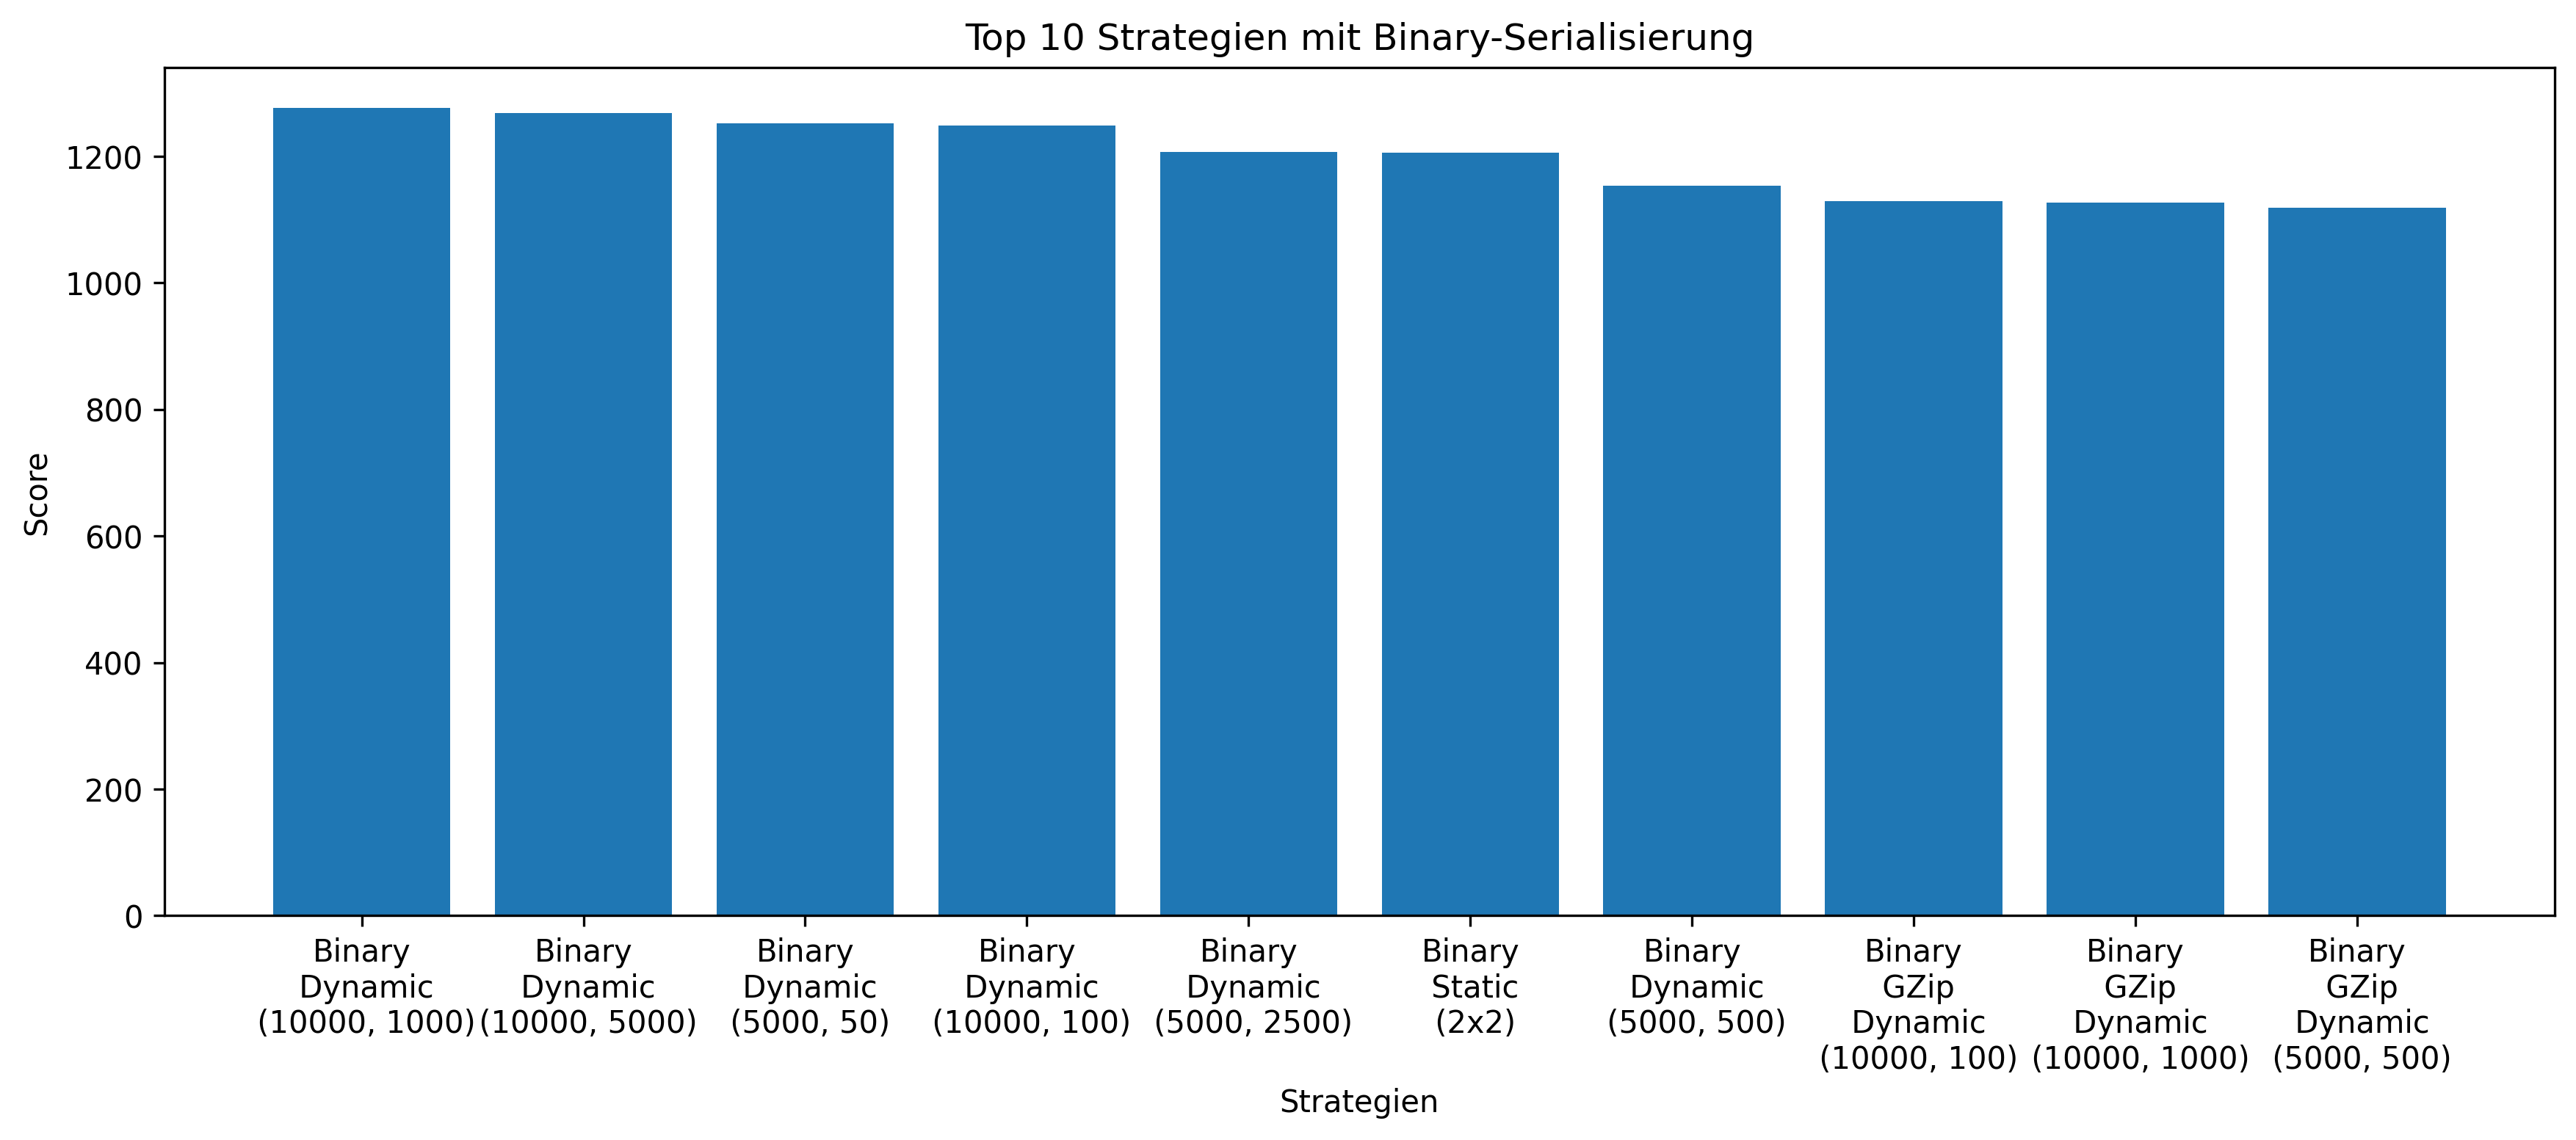
\includegraphics[width=1\textwidth]{images/plots/Binary.png}
    \caption{Beste Binären-Strategien nach dem Score-System aller Kategorien}
    \label{fig:topStratBin}
\end{figure}

\begin{figure}[htp]
    \centering
    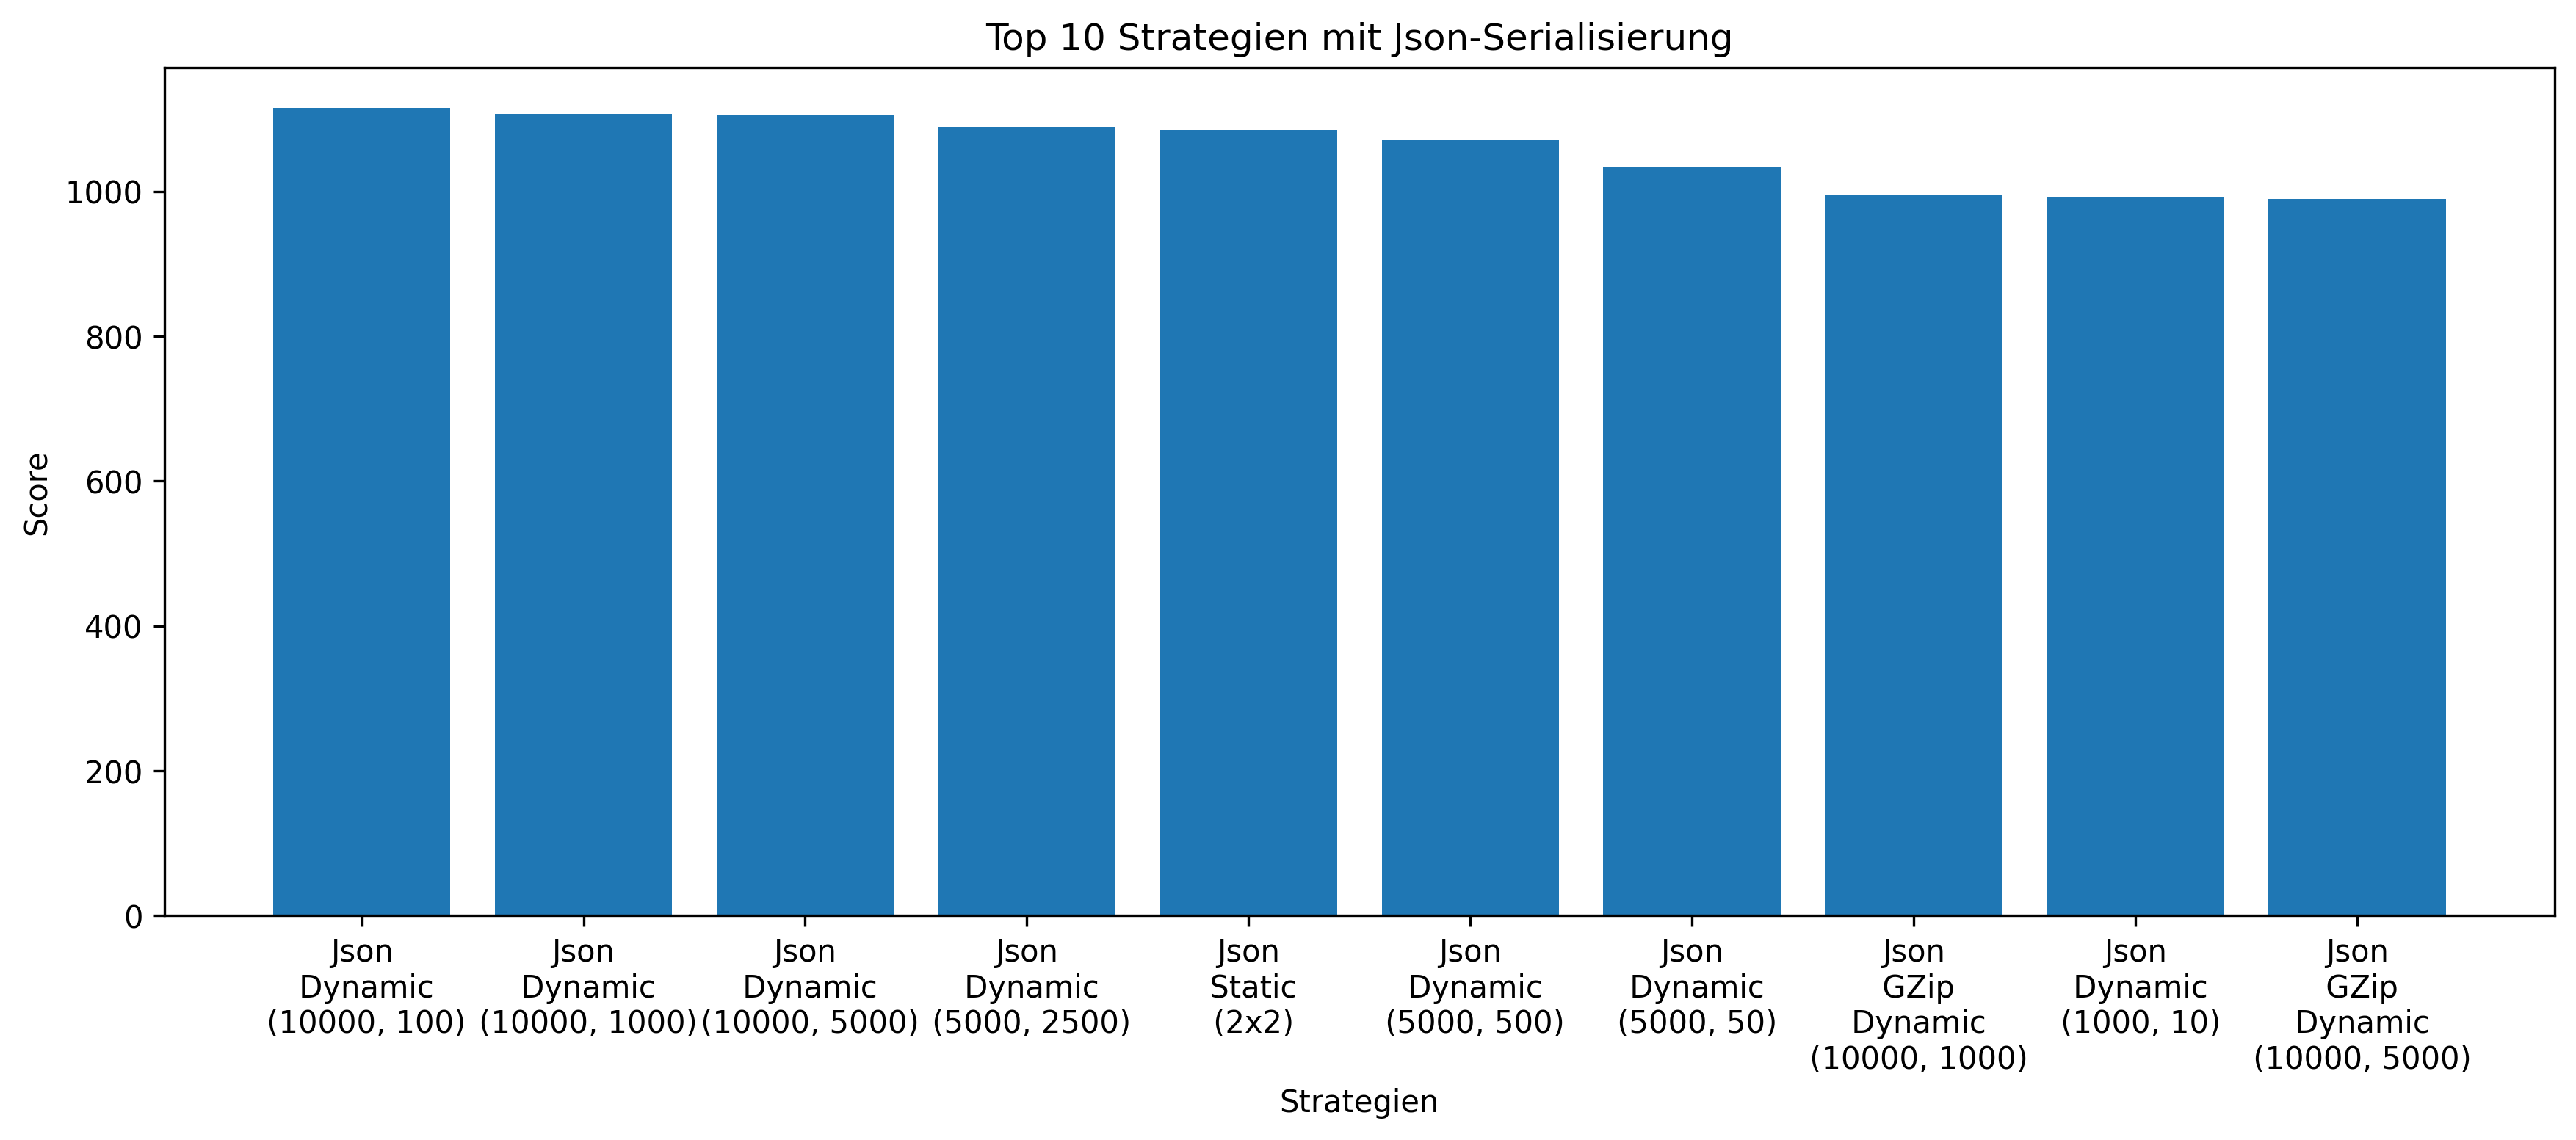
\includegraphics[width=1\textwidth]{images/plots/Json.png}
    \caption{Beste JSON-Strategien nach dem Score-System aller Kategorien}
    \label{fig:topStratJson}
\end{figure}

\begin{figure}[htp]
    \centering
    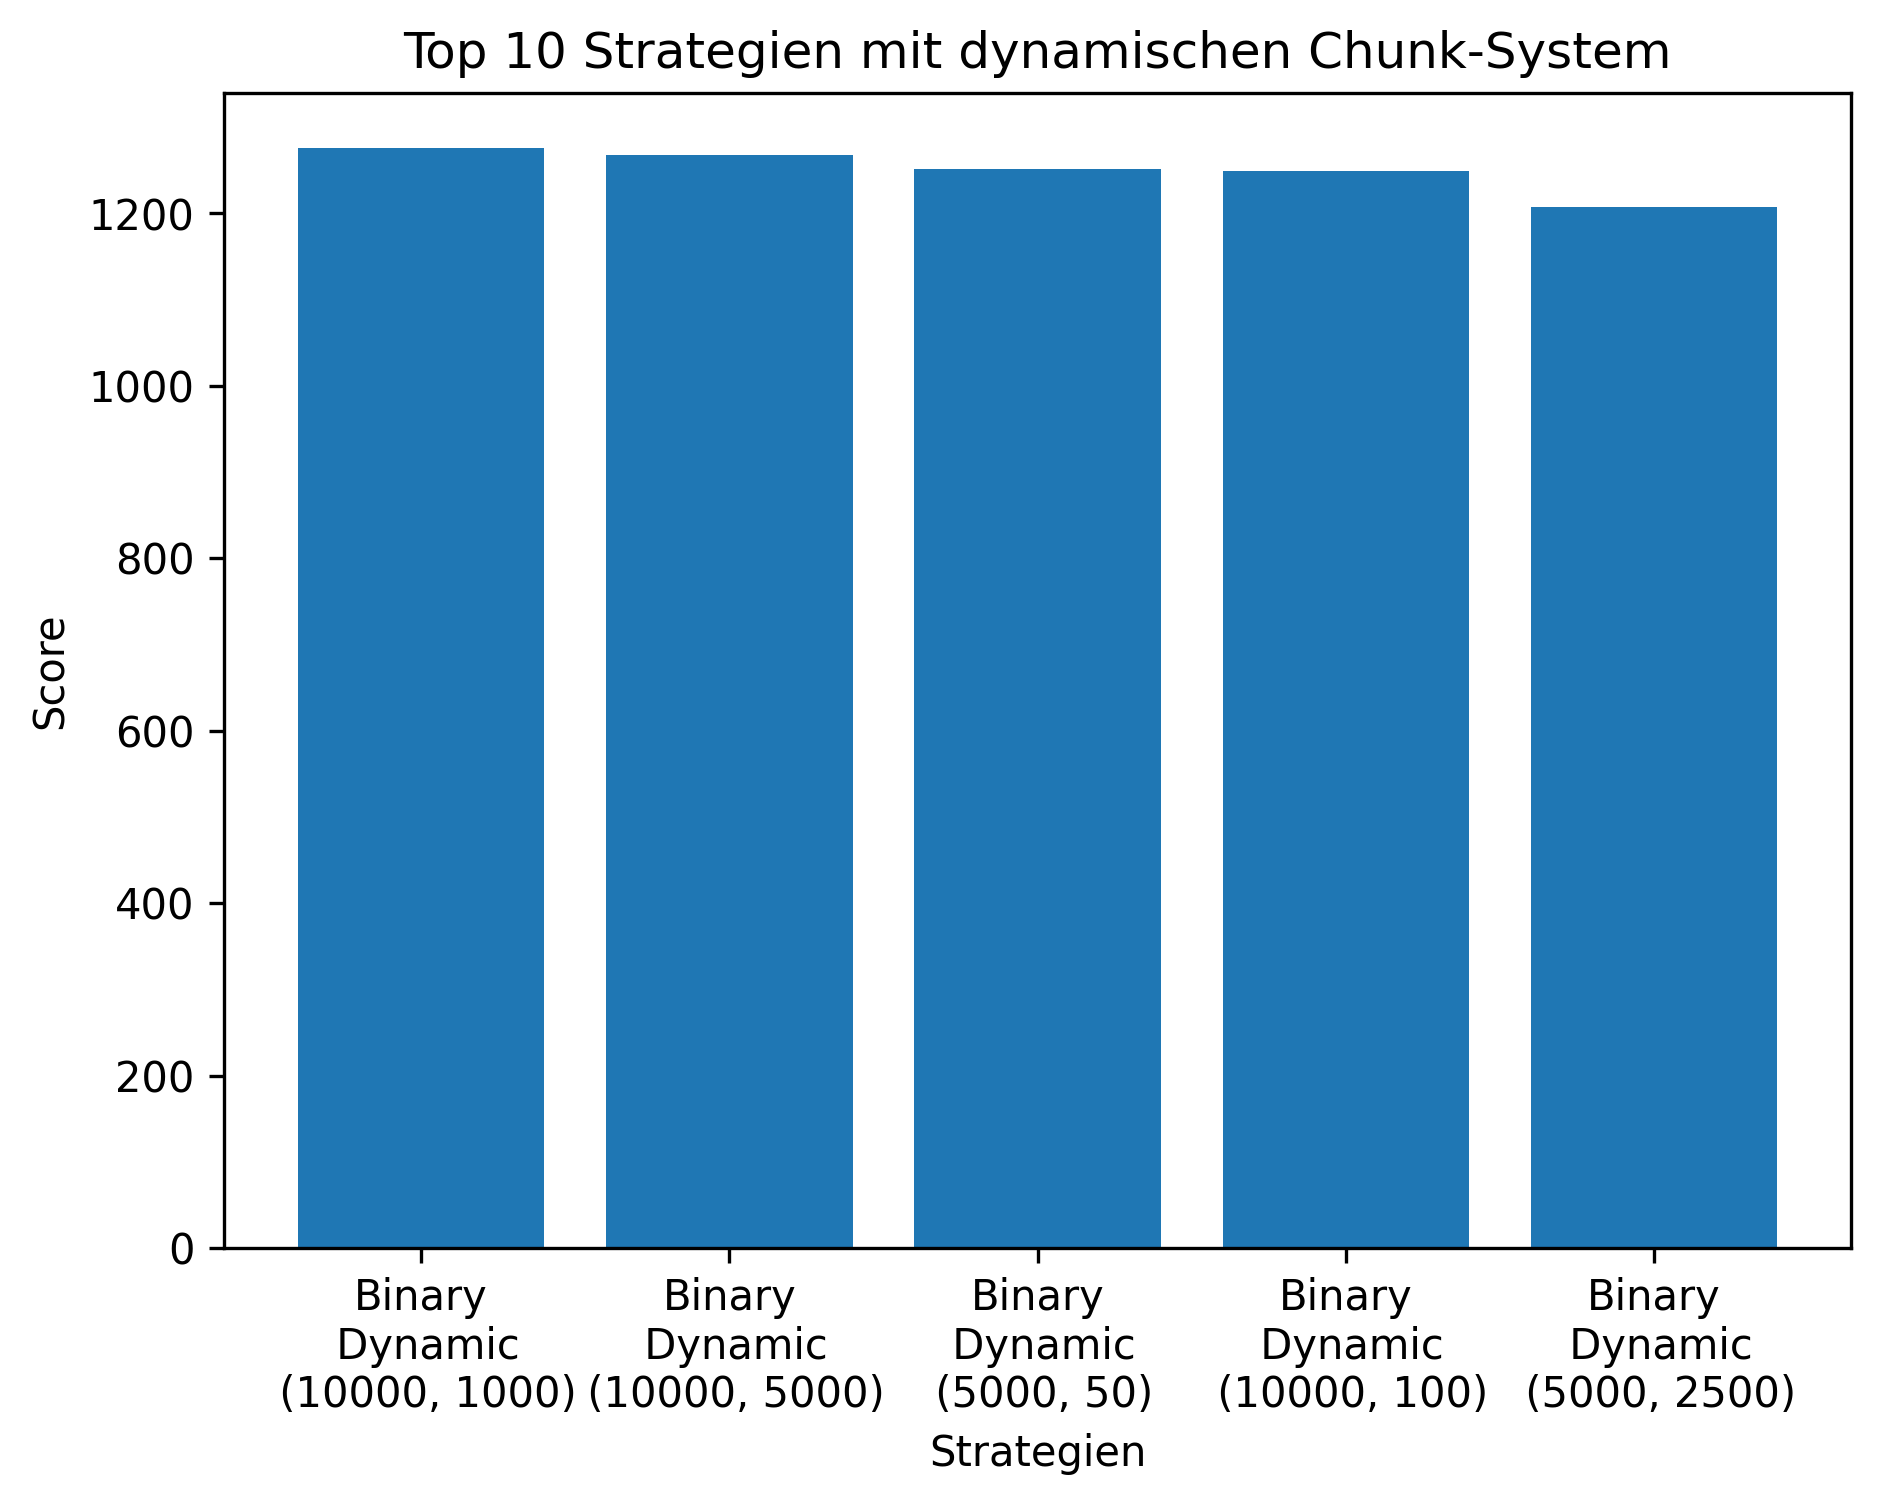
\includegraphics[width=0.7\textwidth]{images/plots/dynamisch.png}
    \caption{Beste Strategien mit dynamischen Chunk-System nach dem Score-System aller Kategorien}
    \label{fig:topDynamic}
\end{figure}

\begin{figure}[htp]
    \centering
    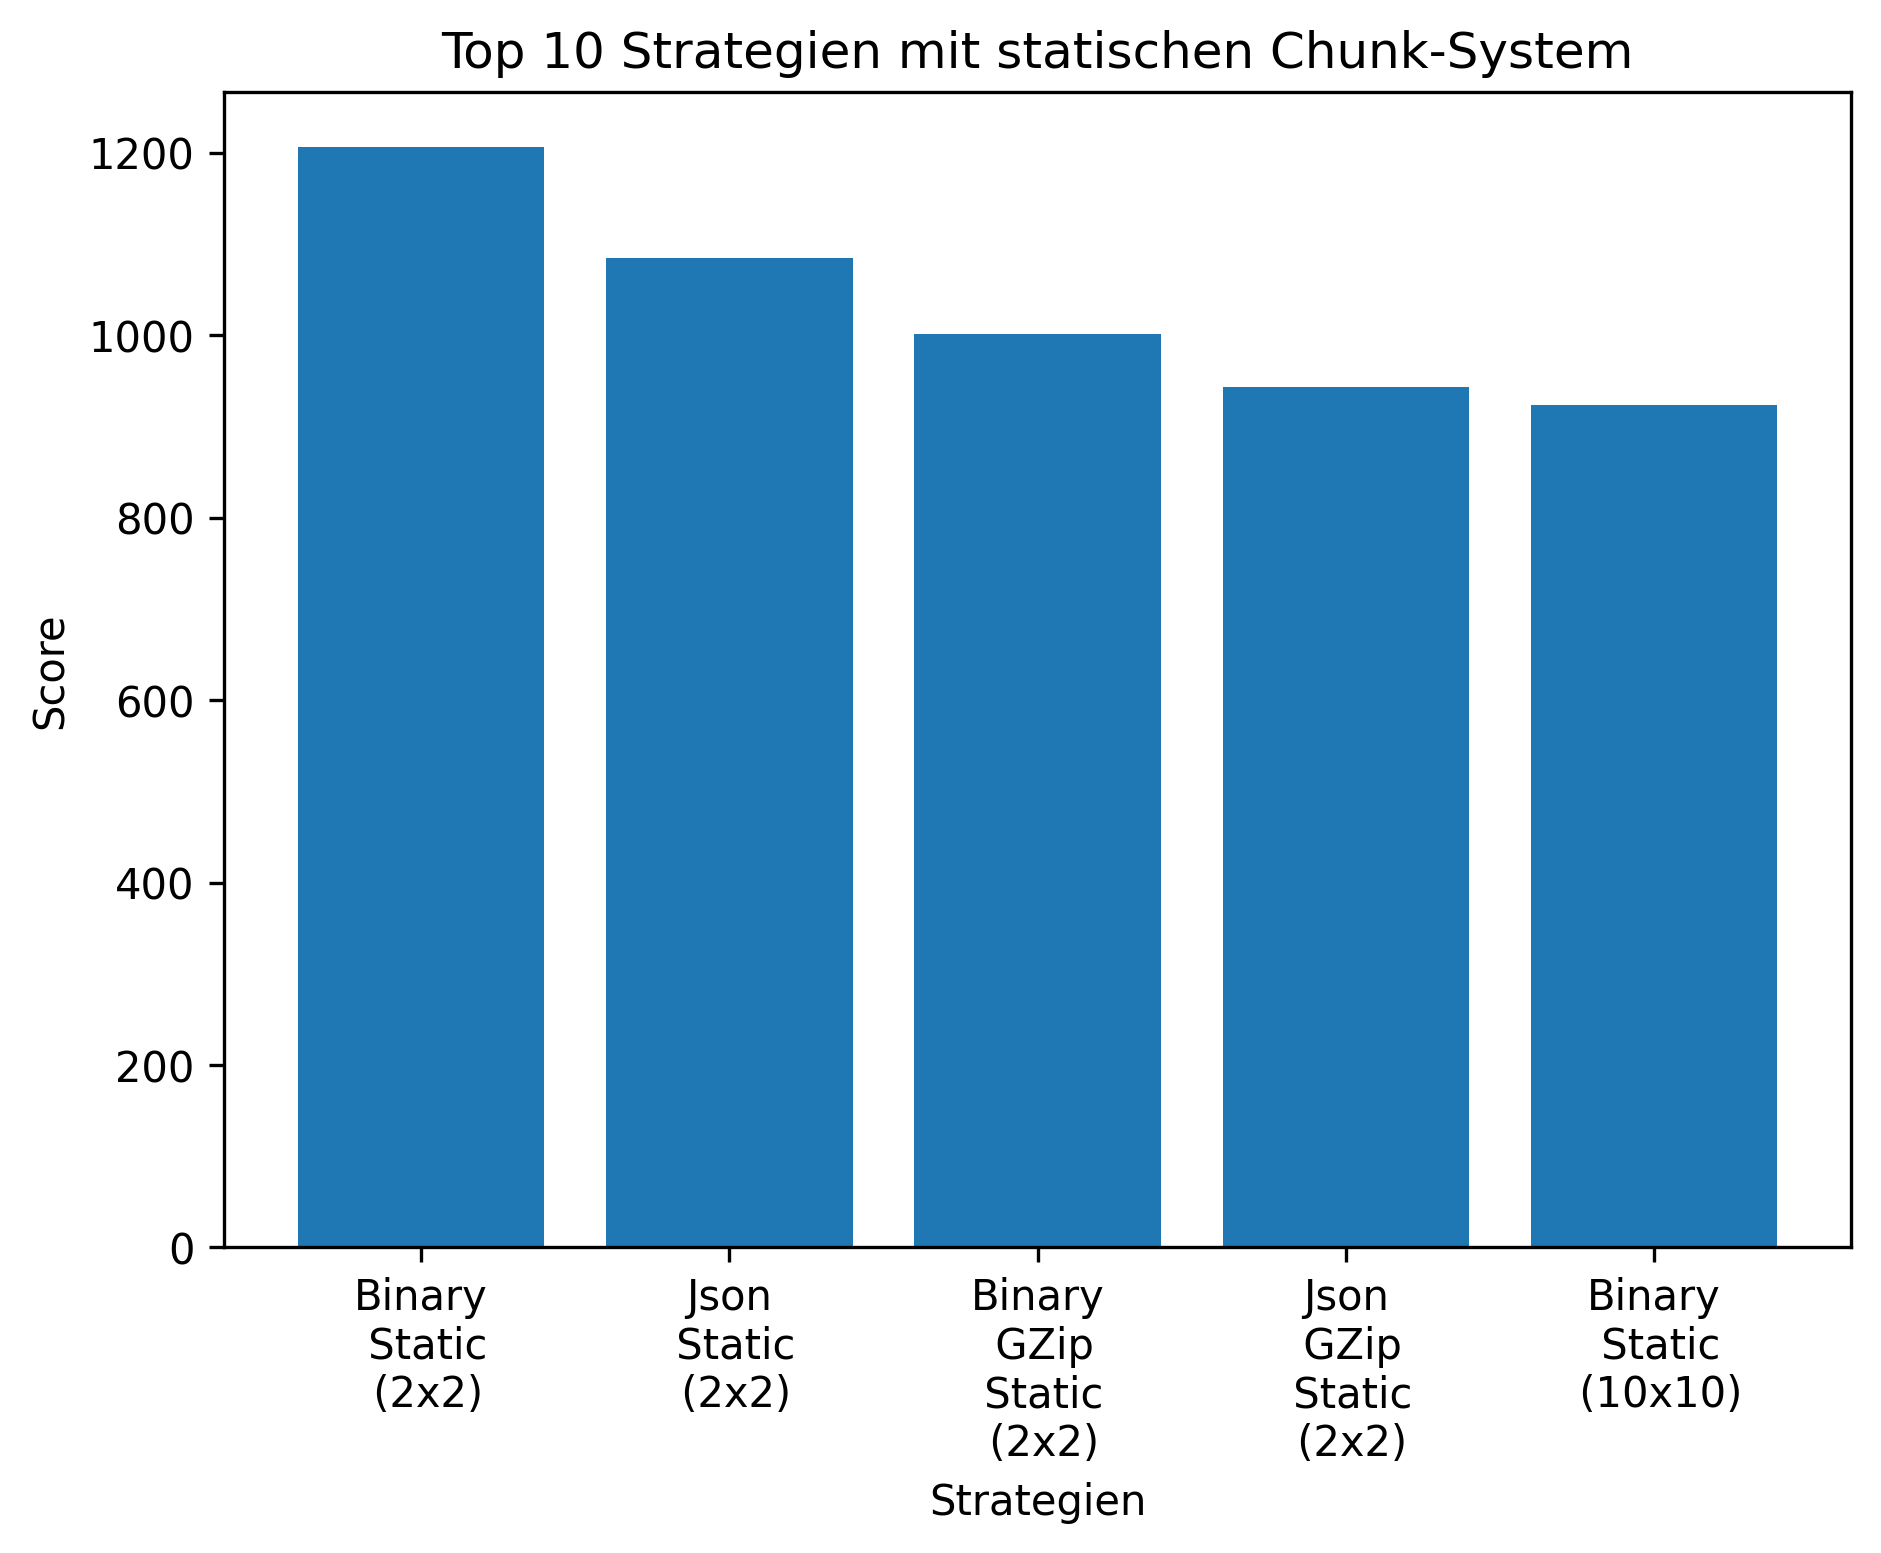
\includegraphics[width=0.7\textwidth]{images/plots/statisch.png}
    \caption{Beste Strategien mit statischen Chunk-System nach dem Score-System aller Kategorien}
    \label{fig:topStatic}
\end{figure}

\begin{figure}[htp]
    \centering
    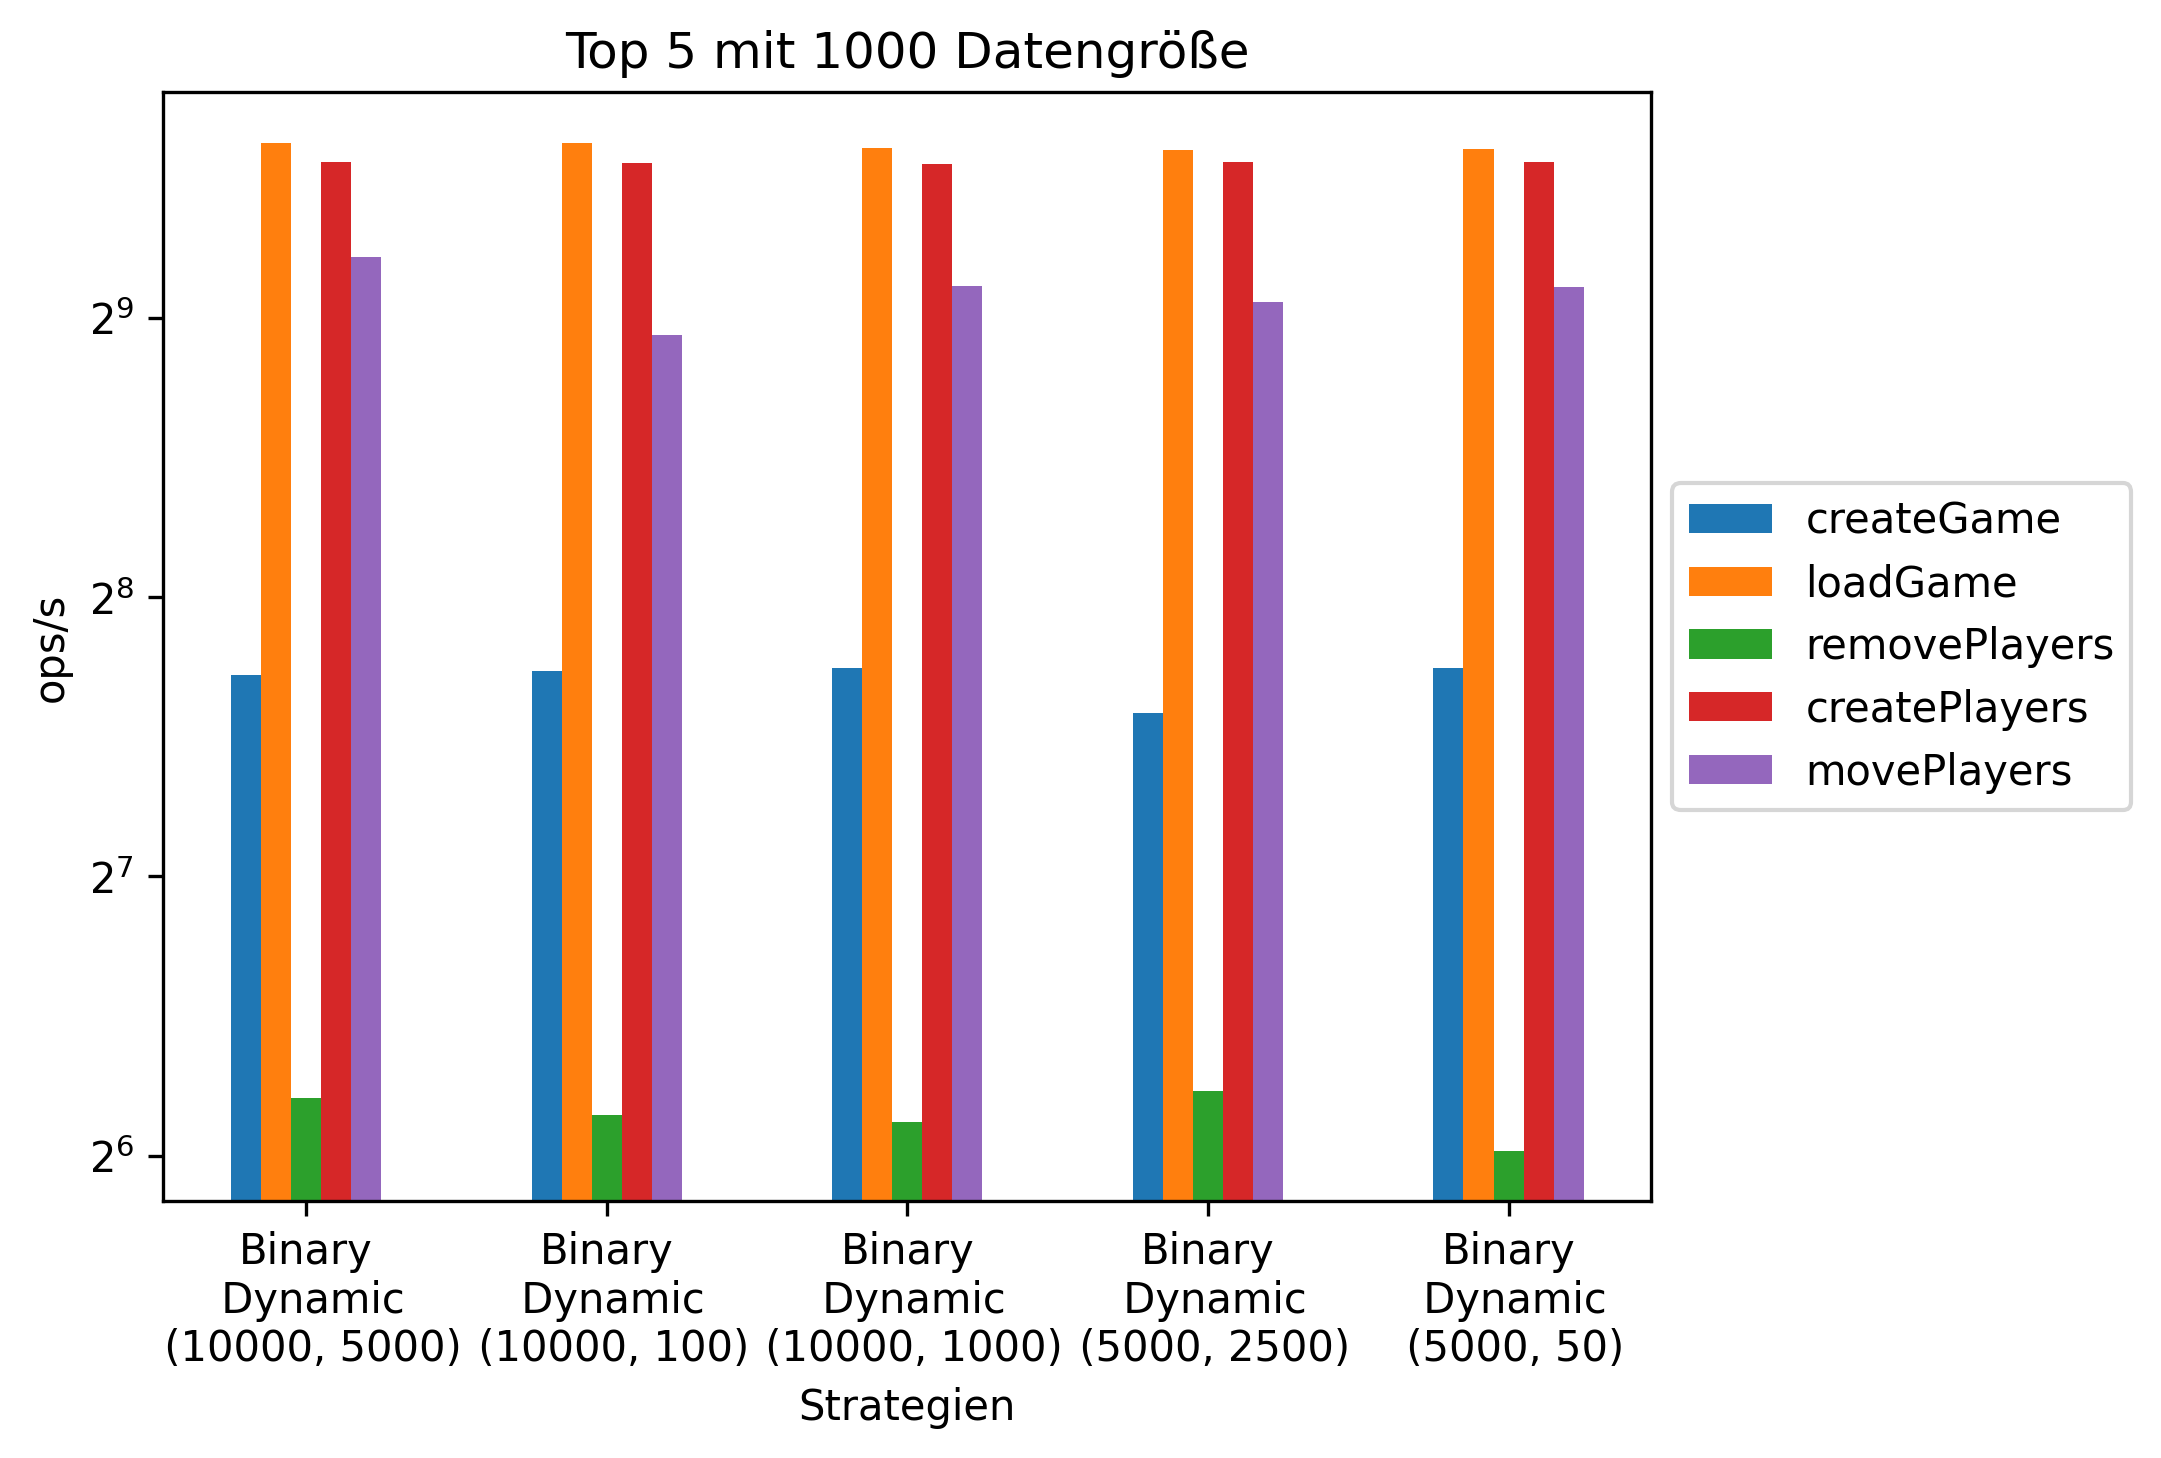
\includegraphics[width=0.7\textwidth]{images/plots/1000.png}
    \caption{Beste Strategien bei einer Datengröße von 1000}
    \label{fig:smallDataCount}
\end{figure}

\begin{figure}[htp]
    \centering
    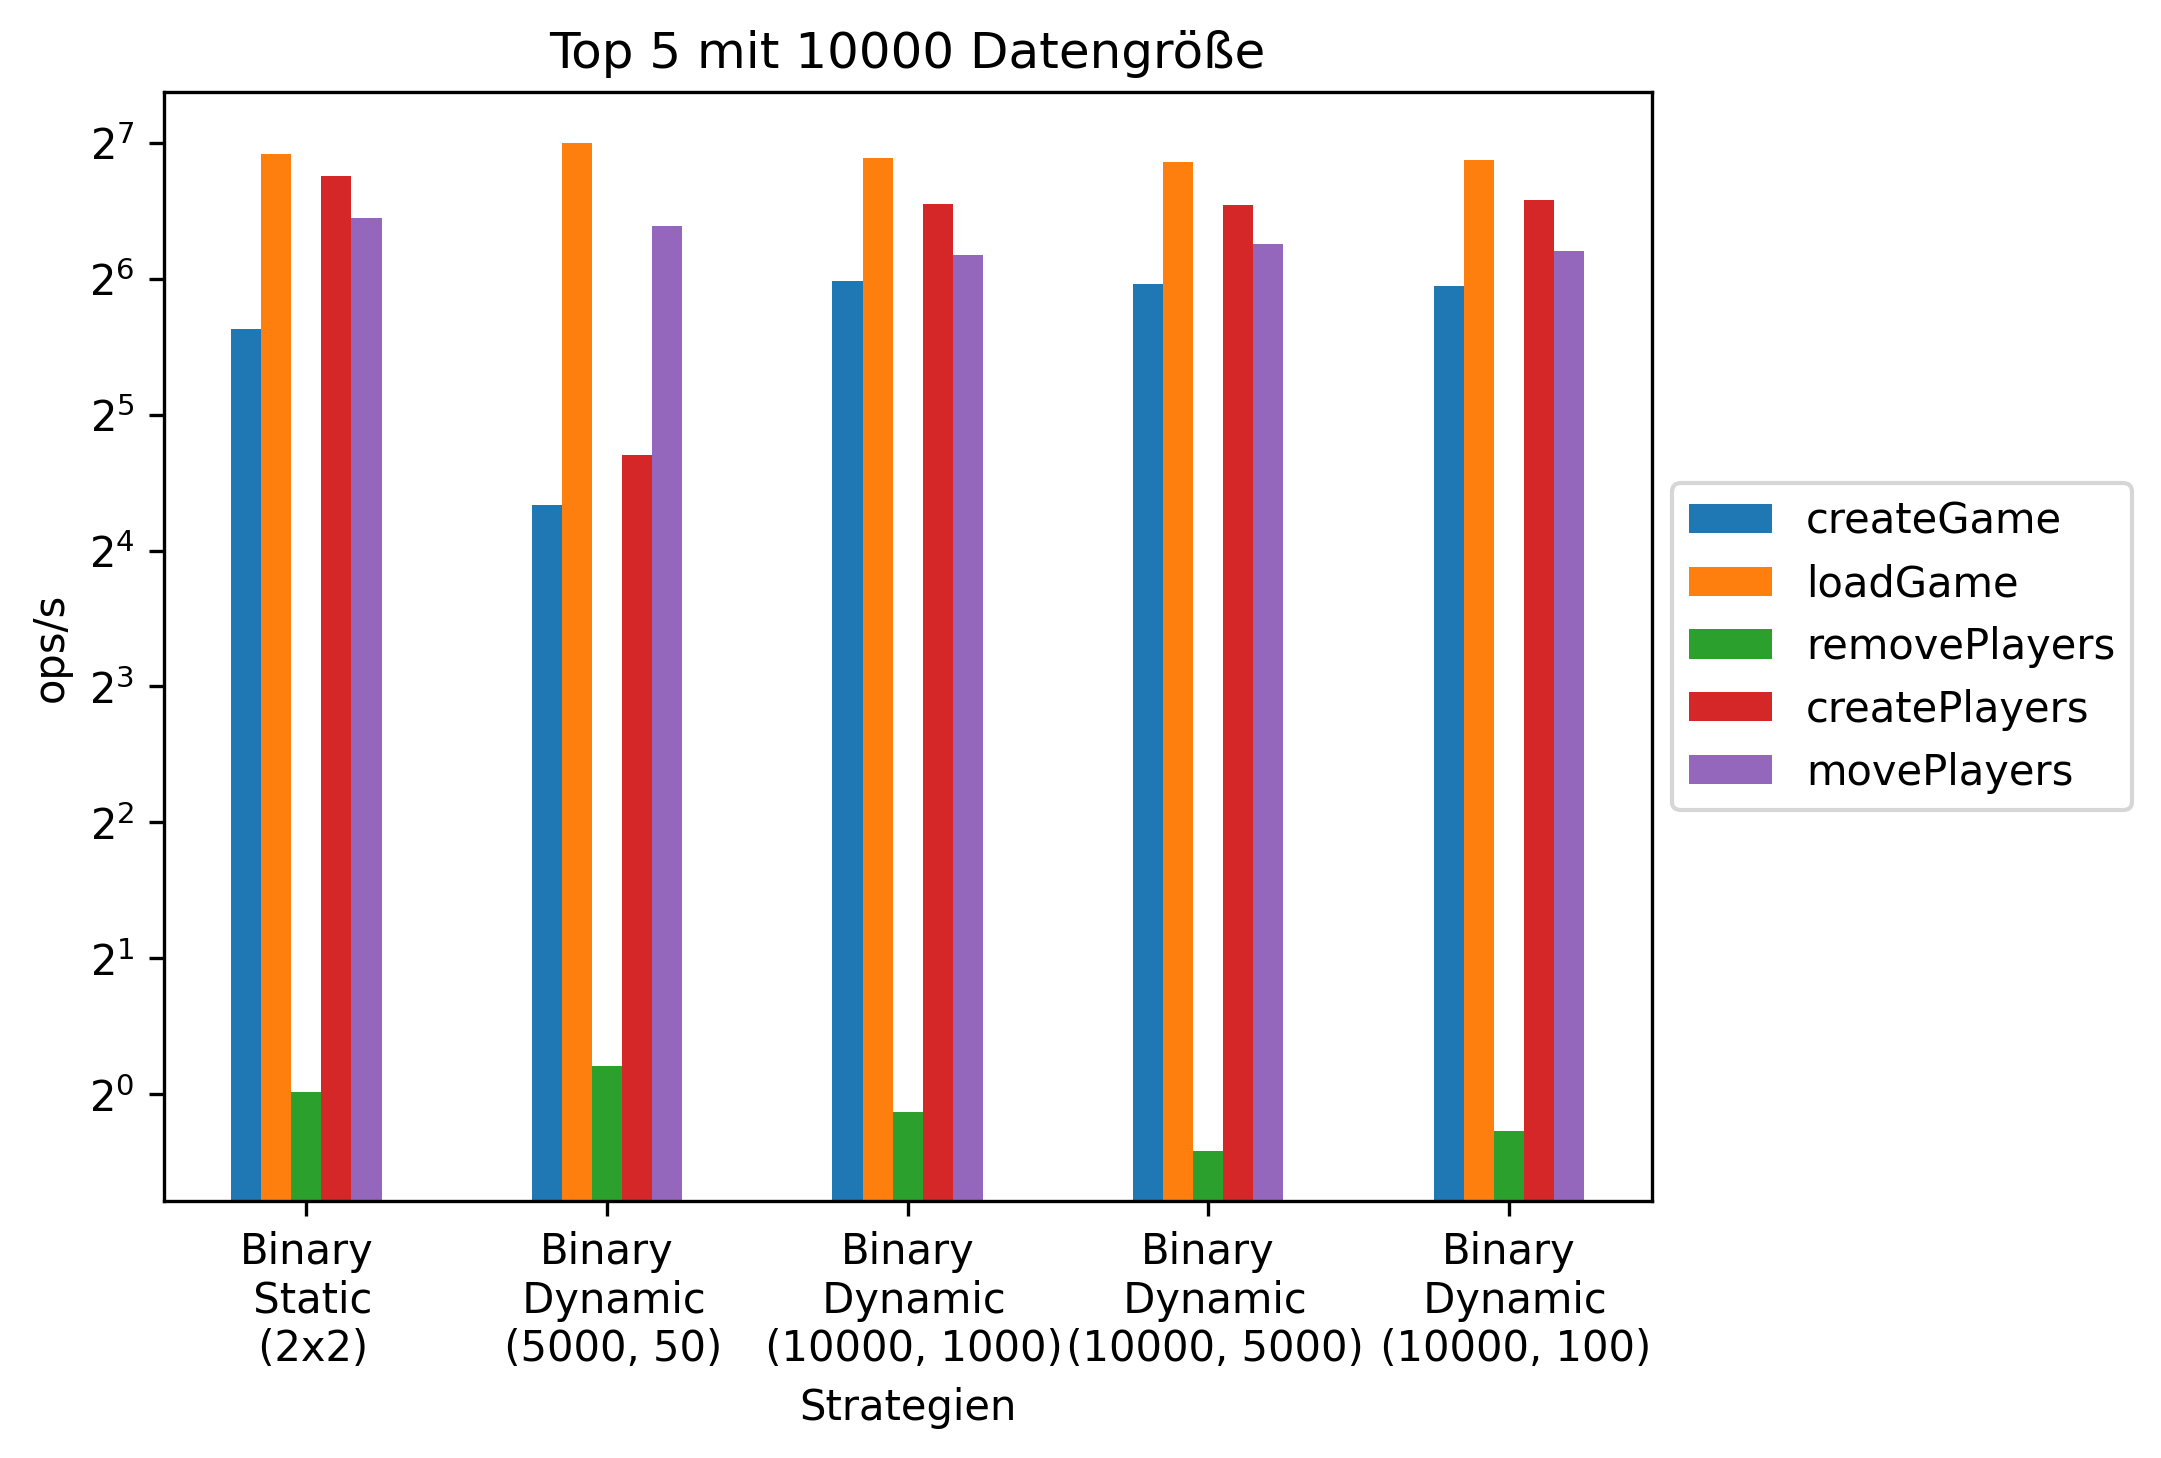
\includegraphics[width=0.7\textwidth]{images/plots/10000.png}
    \caption{Beste Strategien bei einer Datengröße von 10000}
    \label{fig:middleDataCount}
\end{figure}

\begin{figure}[htp]
    \centering
    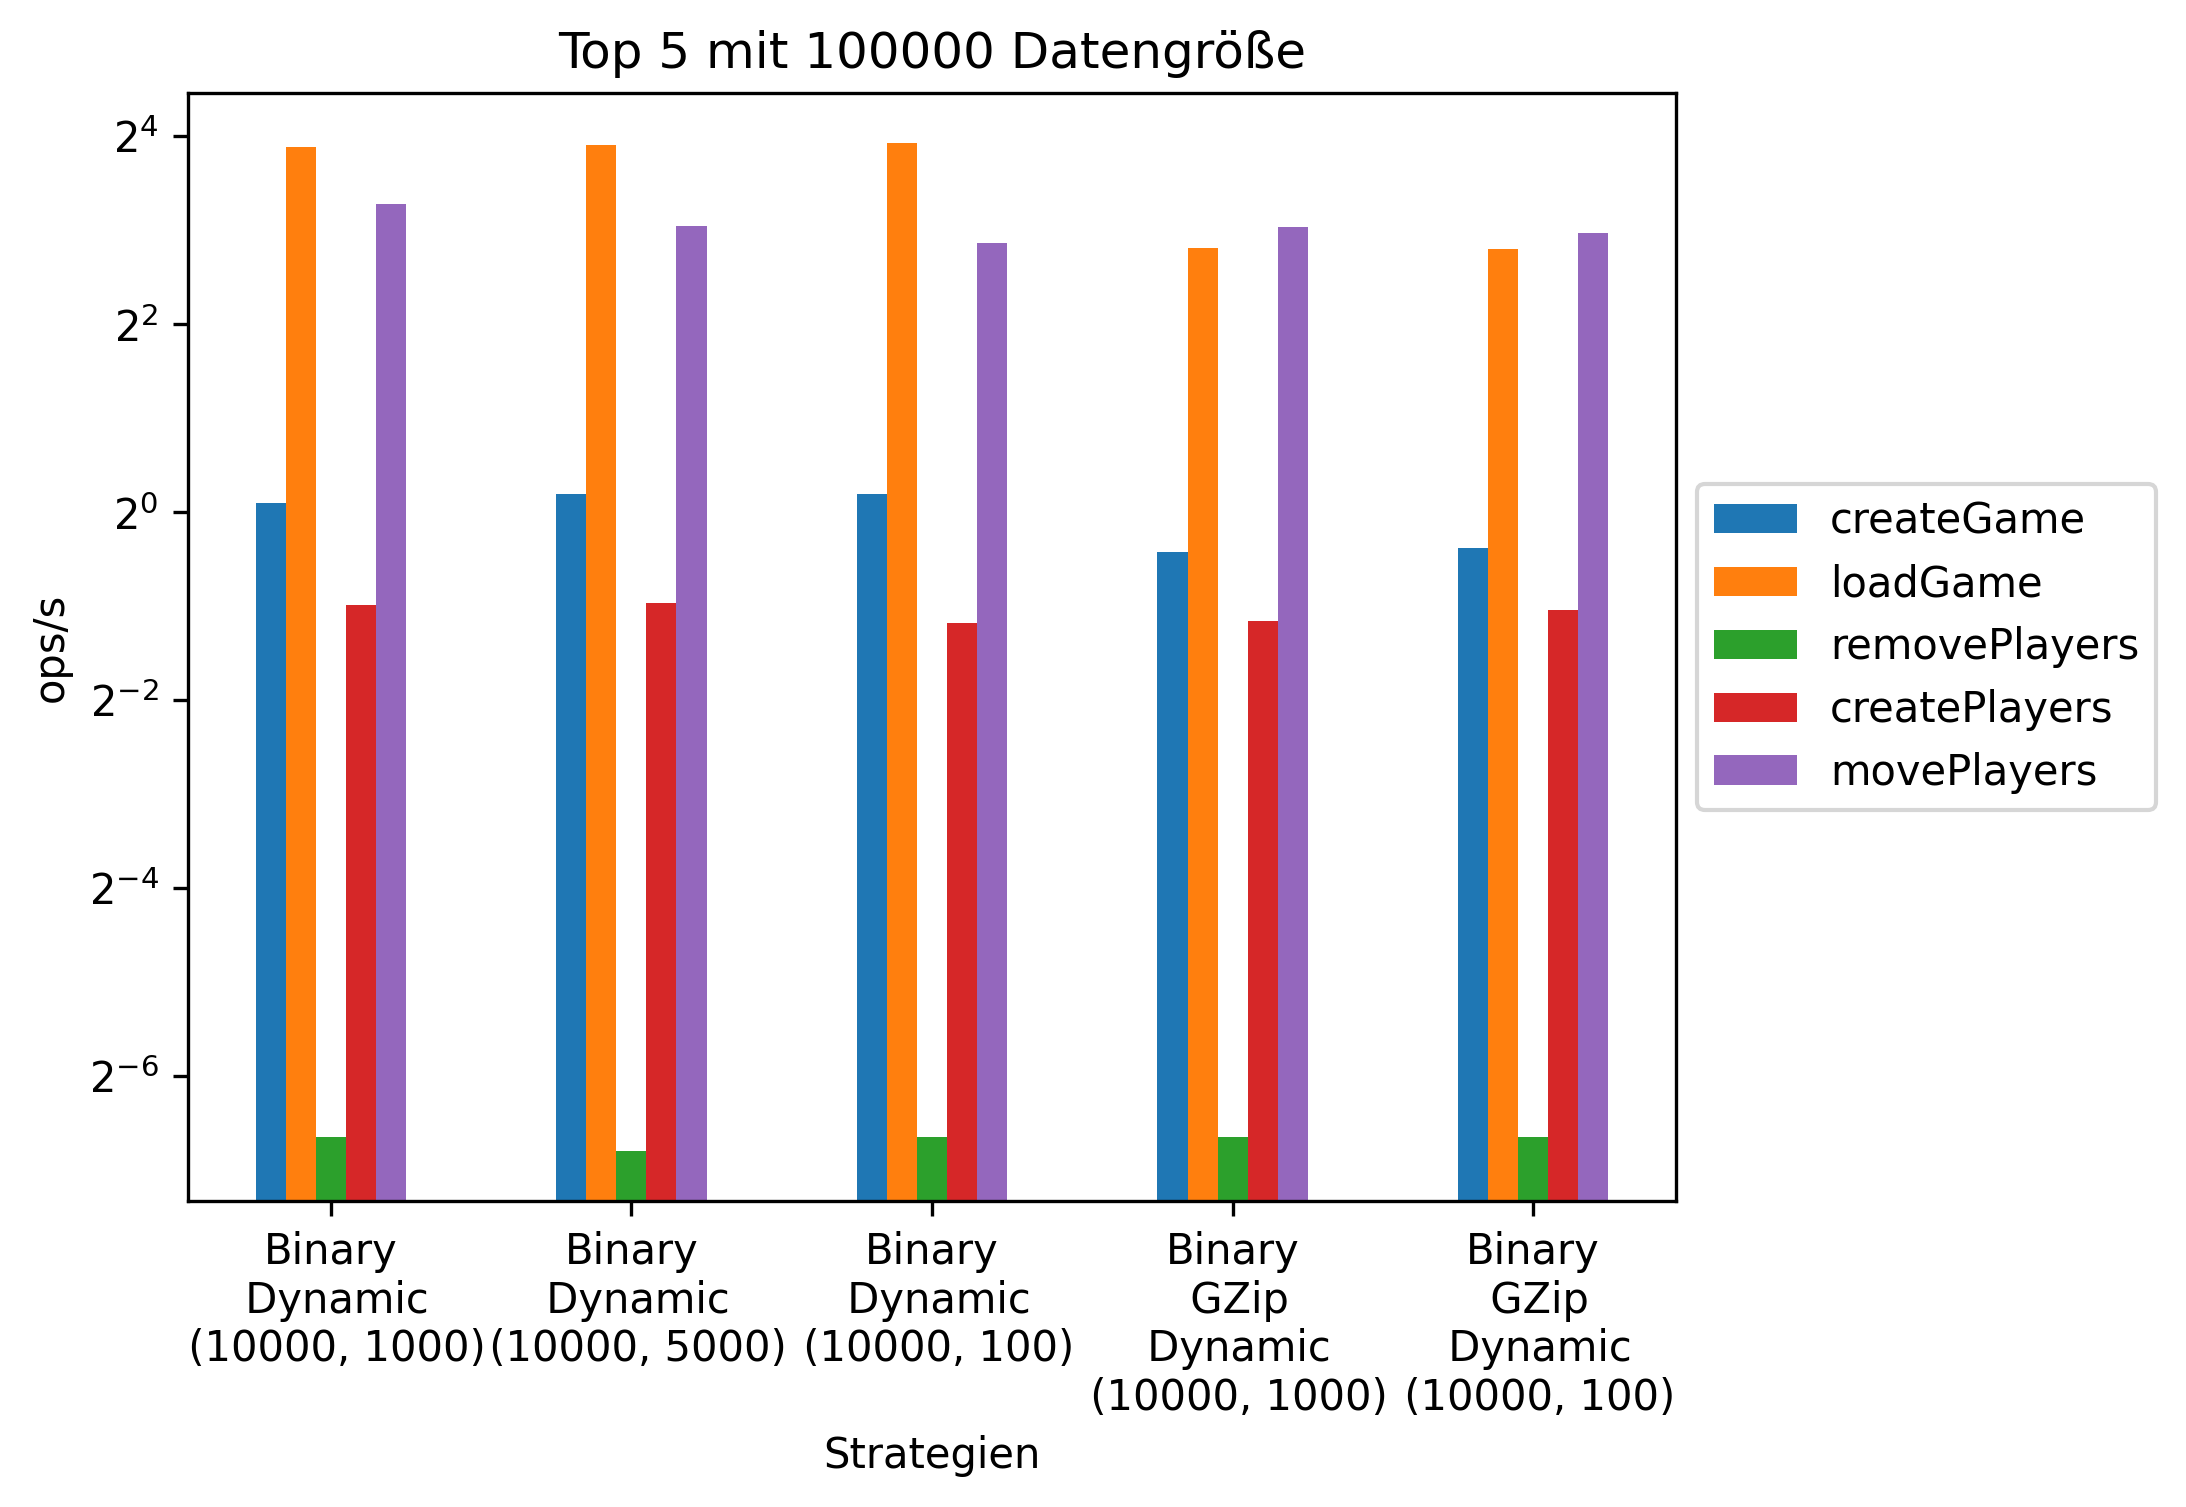
\includegraphics[width=0.7\textwidth]{images/plots/100000.png}
    \caption{Beste Strategien bei einer Daten-Anzahl von 100000}
    \label{fig:bigDataCount}
\end{figure}

\begin{figure}[htp]
    \centering
    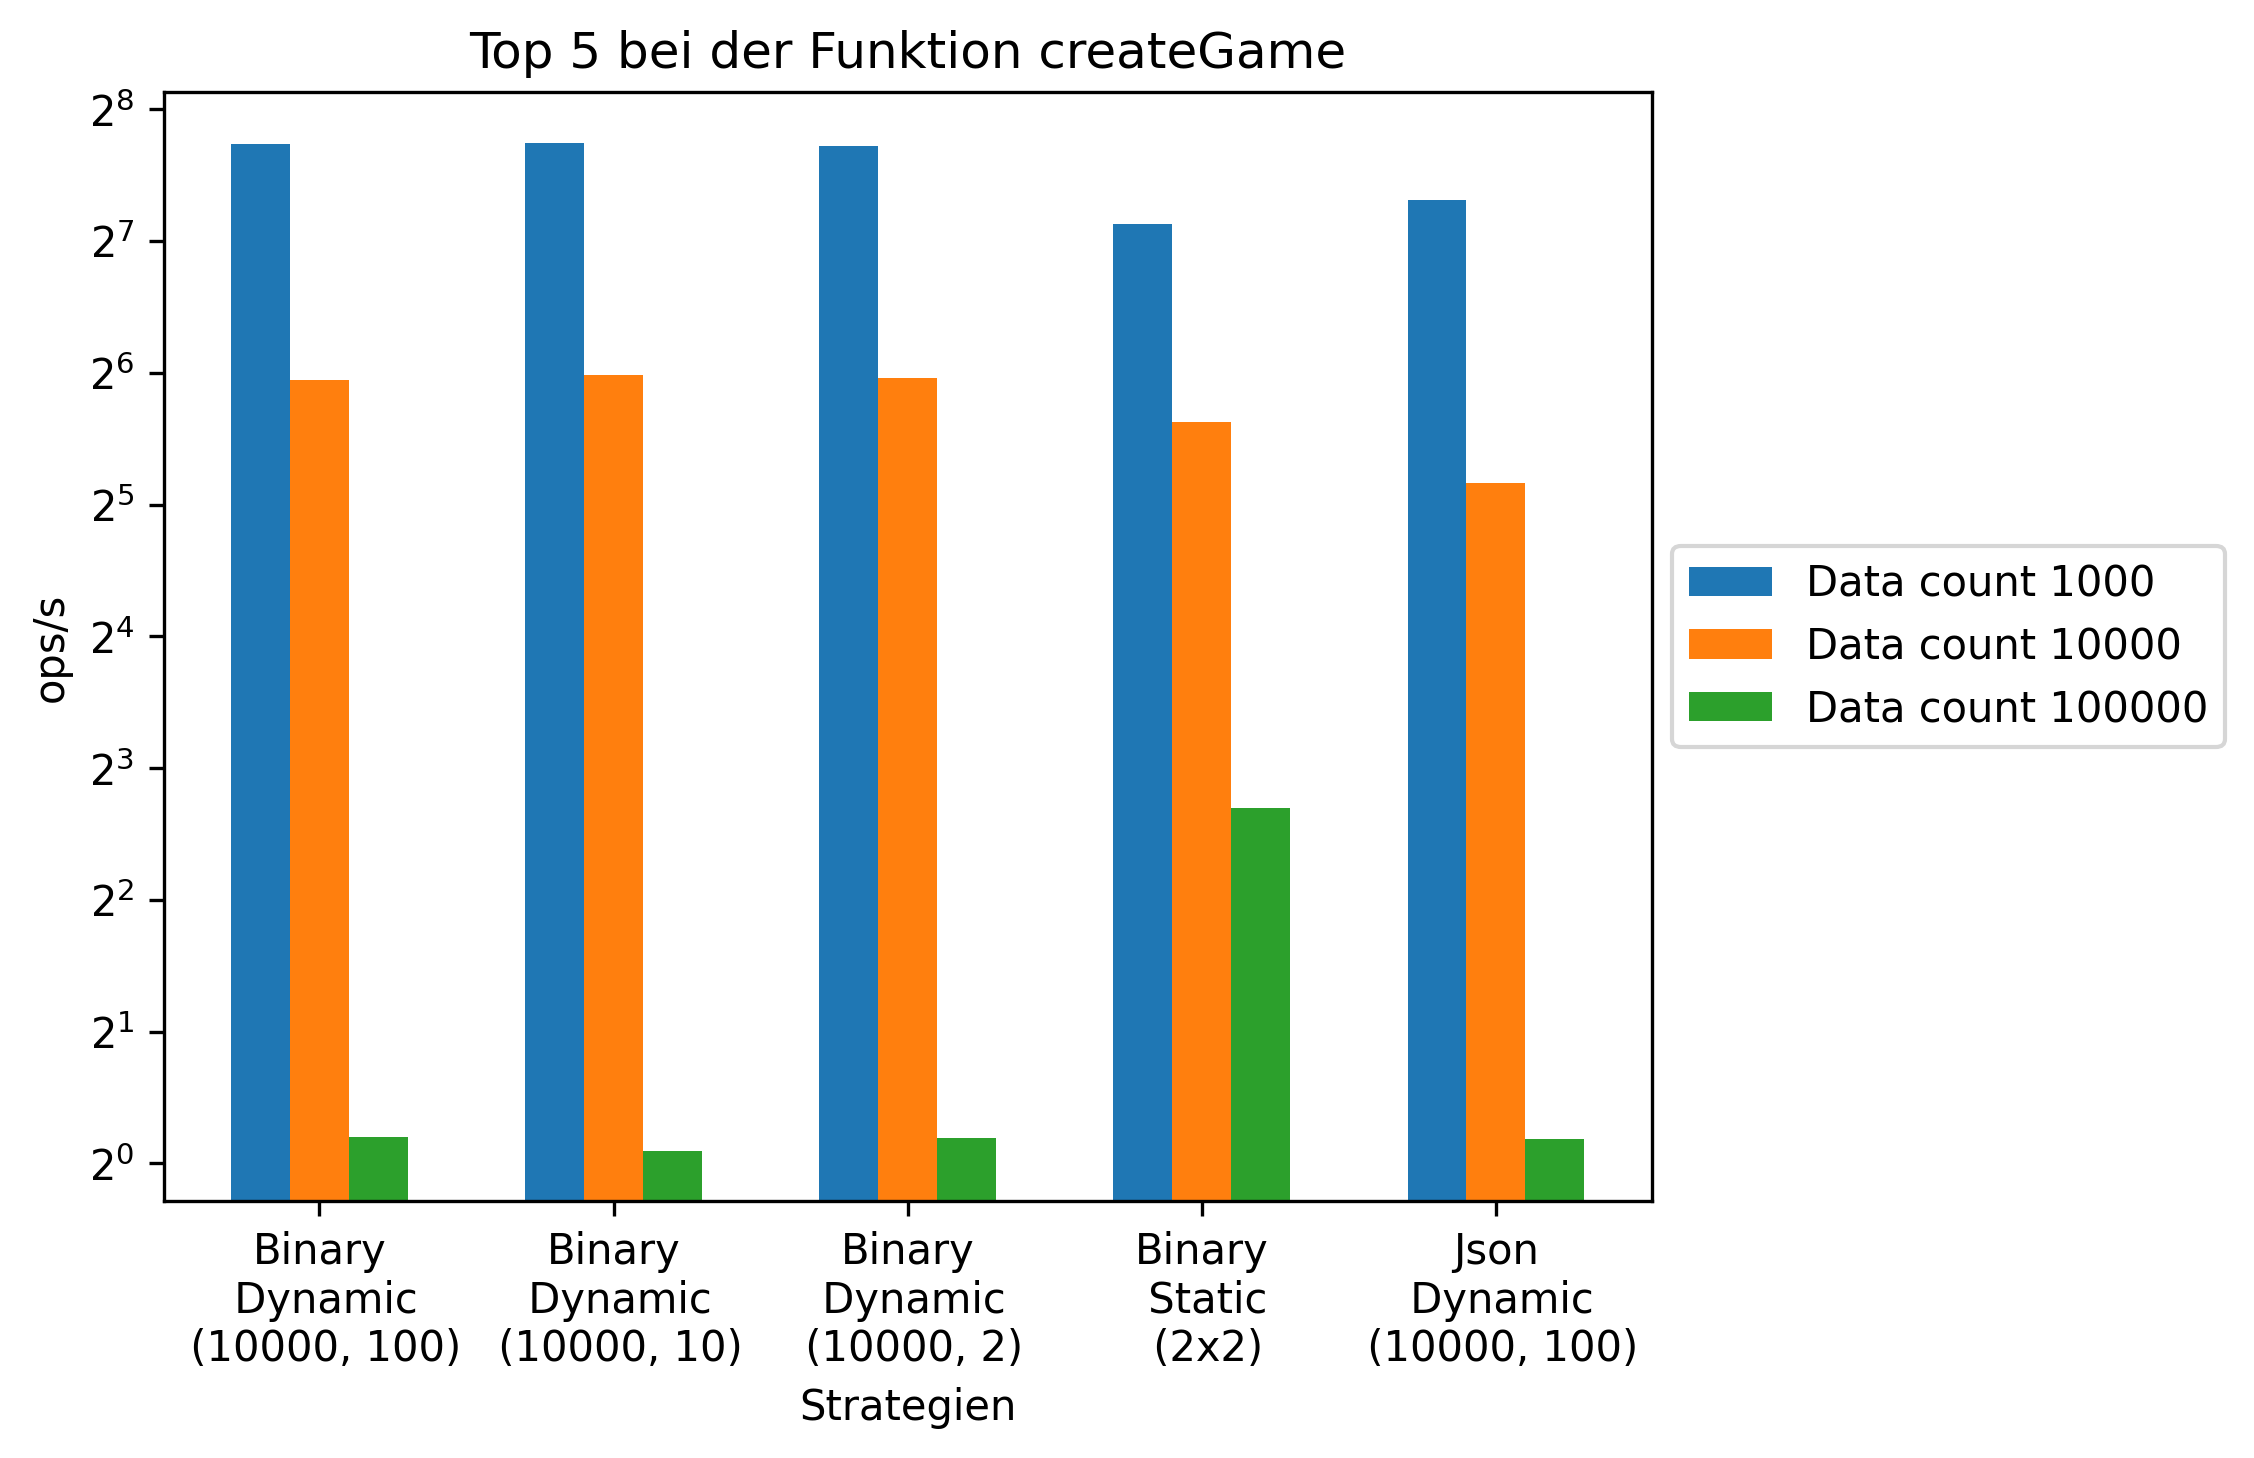
\includegraphics[width=0.7\textwidth]{images/plots/createGame.png}
    \caption{Beste Strategien für die Funktion createGame}
    \label{fig:createGame}
\end{figure}

\begin{figure}[htp]
    \centering
    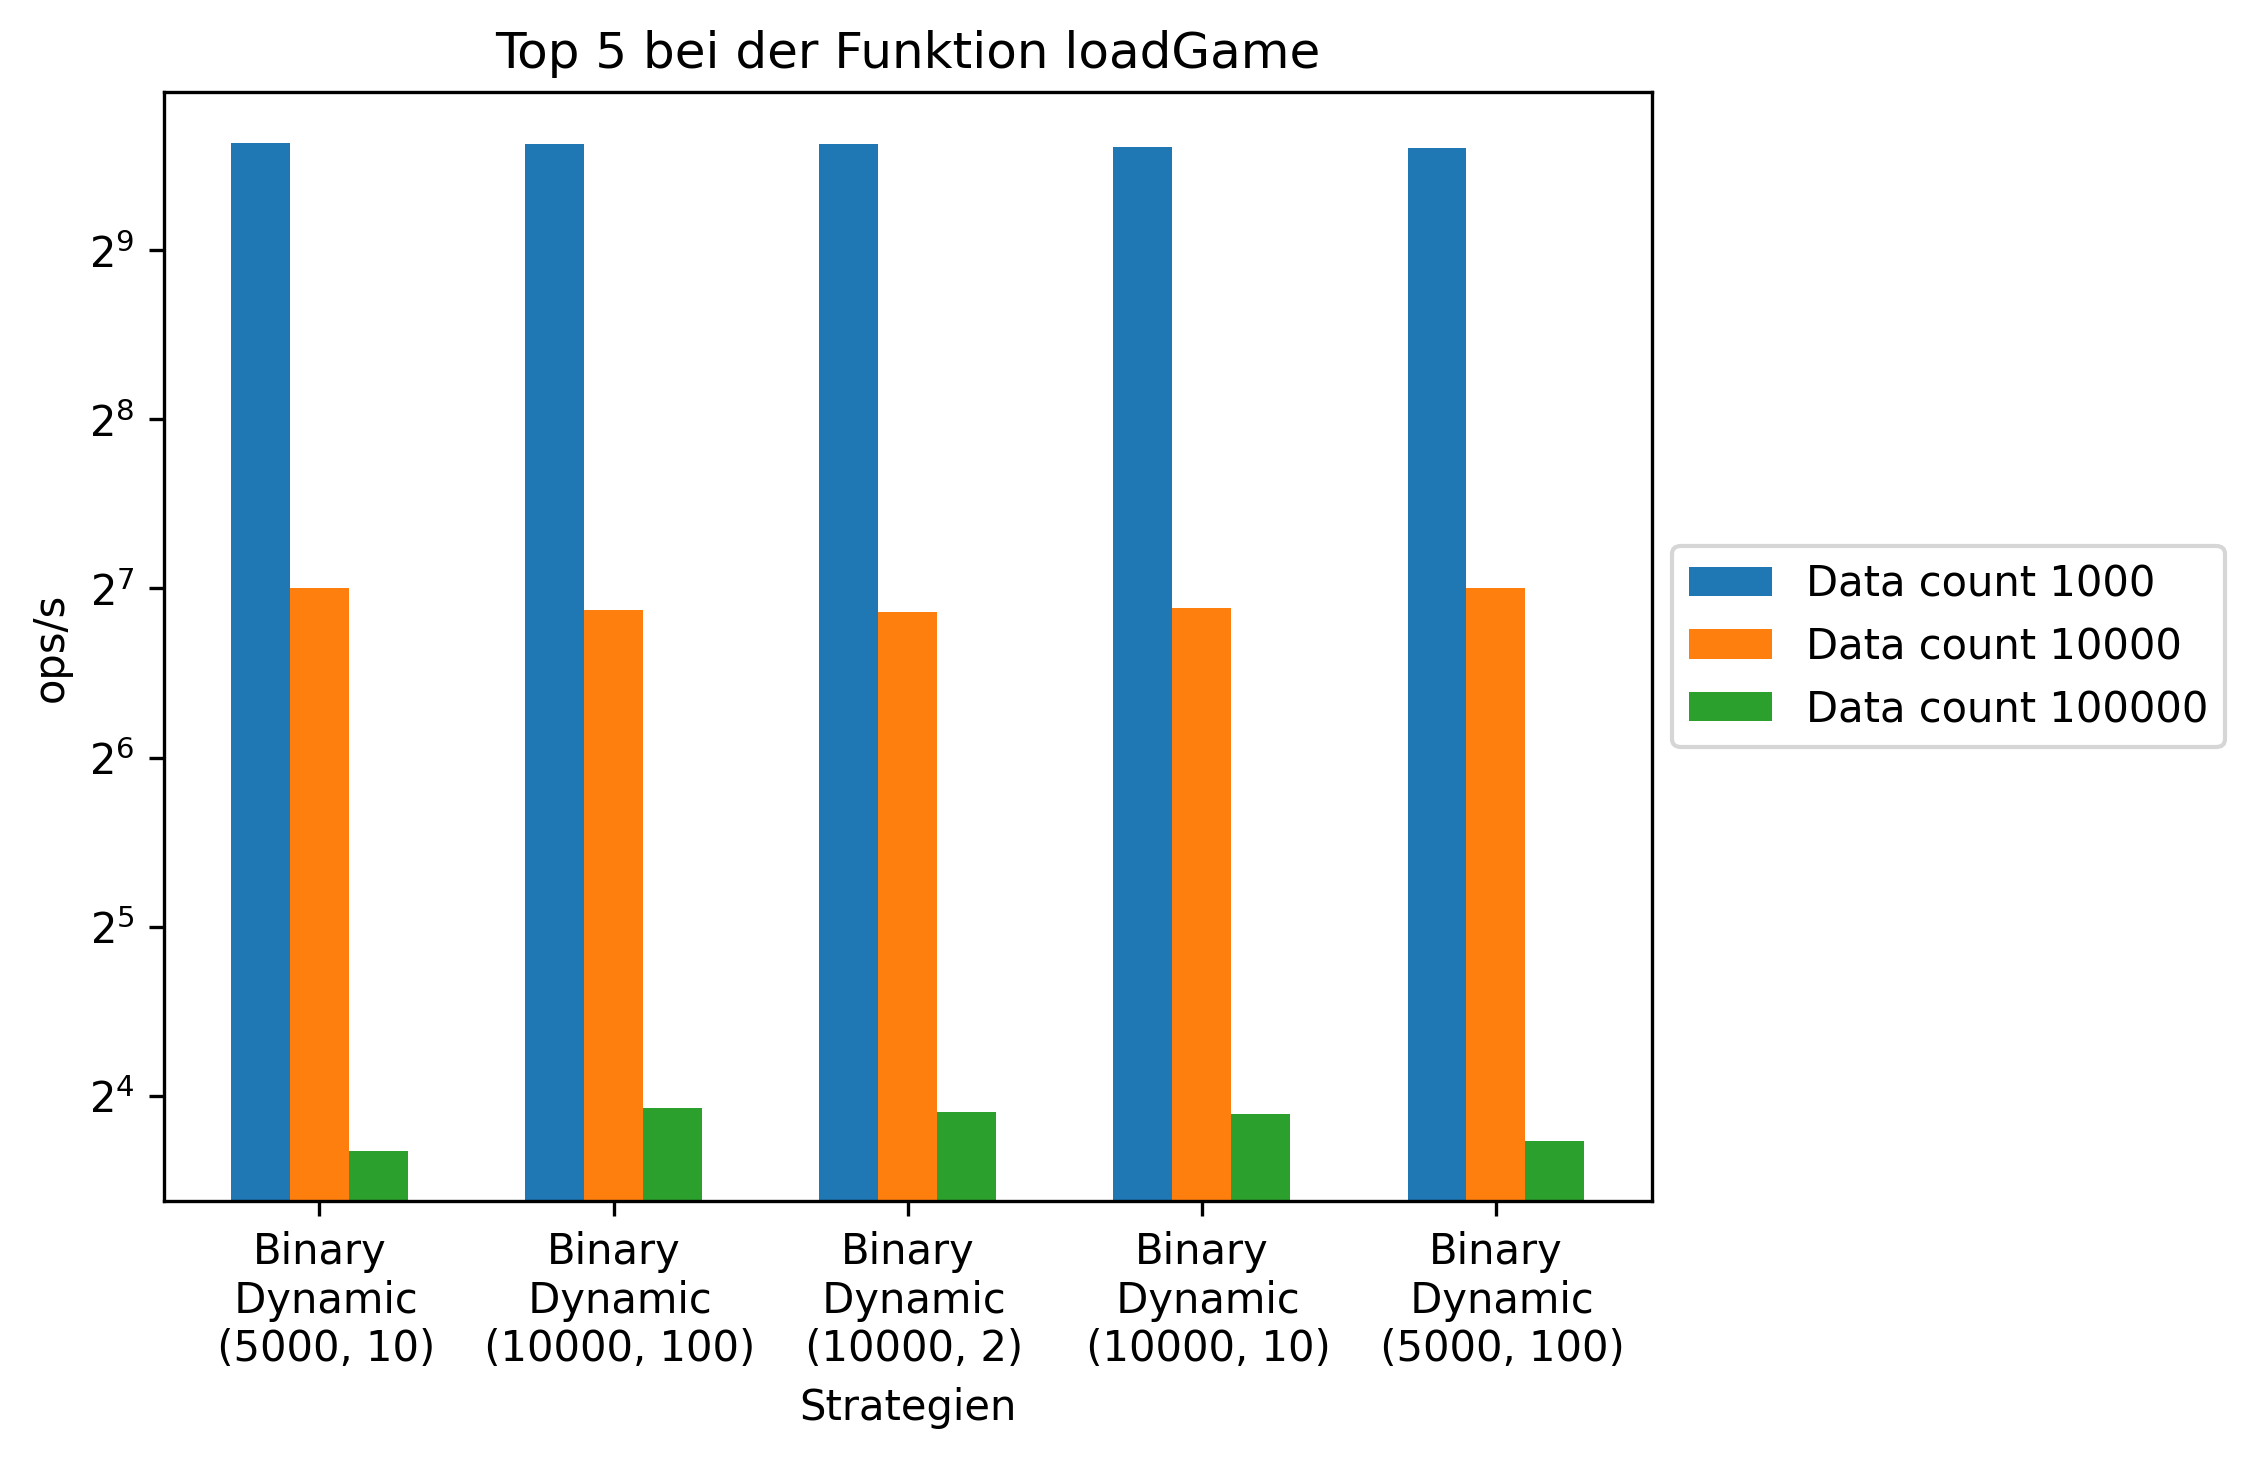
\includegraphics[width=0.7\textwidth]{images/plots/loadGame.png}
    \caption{Beste Strategien für die Funktion loadGame}
    \label{fig:loadGame}
\end{figure}

\begin{figure}[htp]
    \centering
    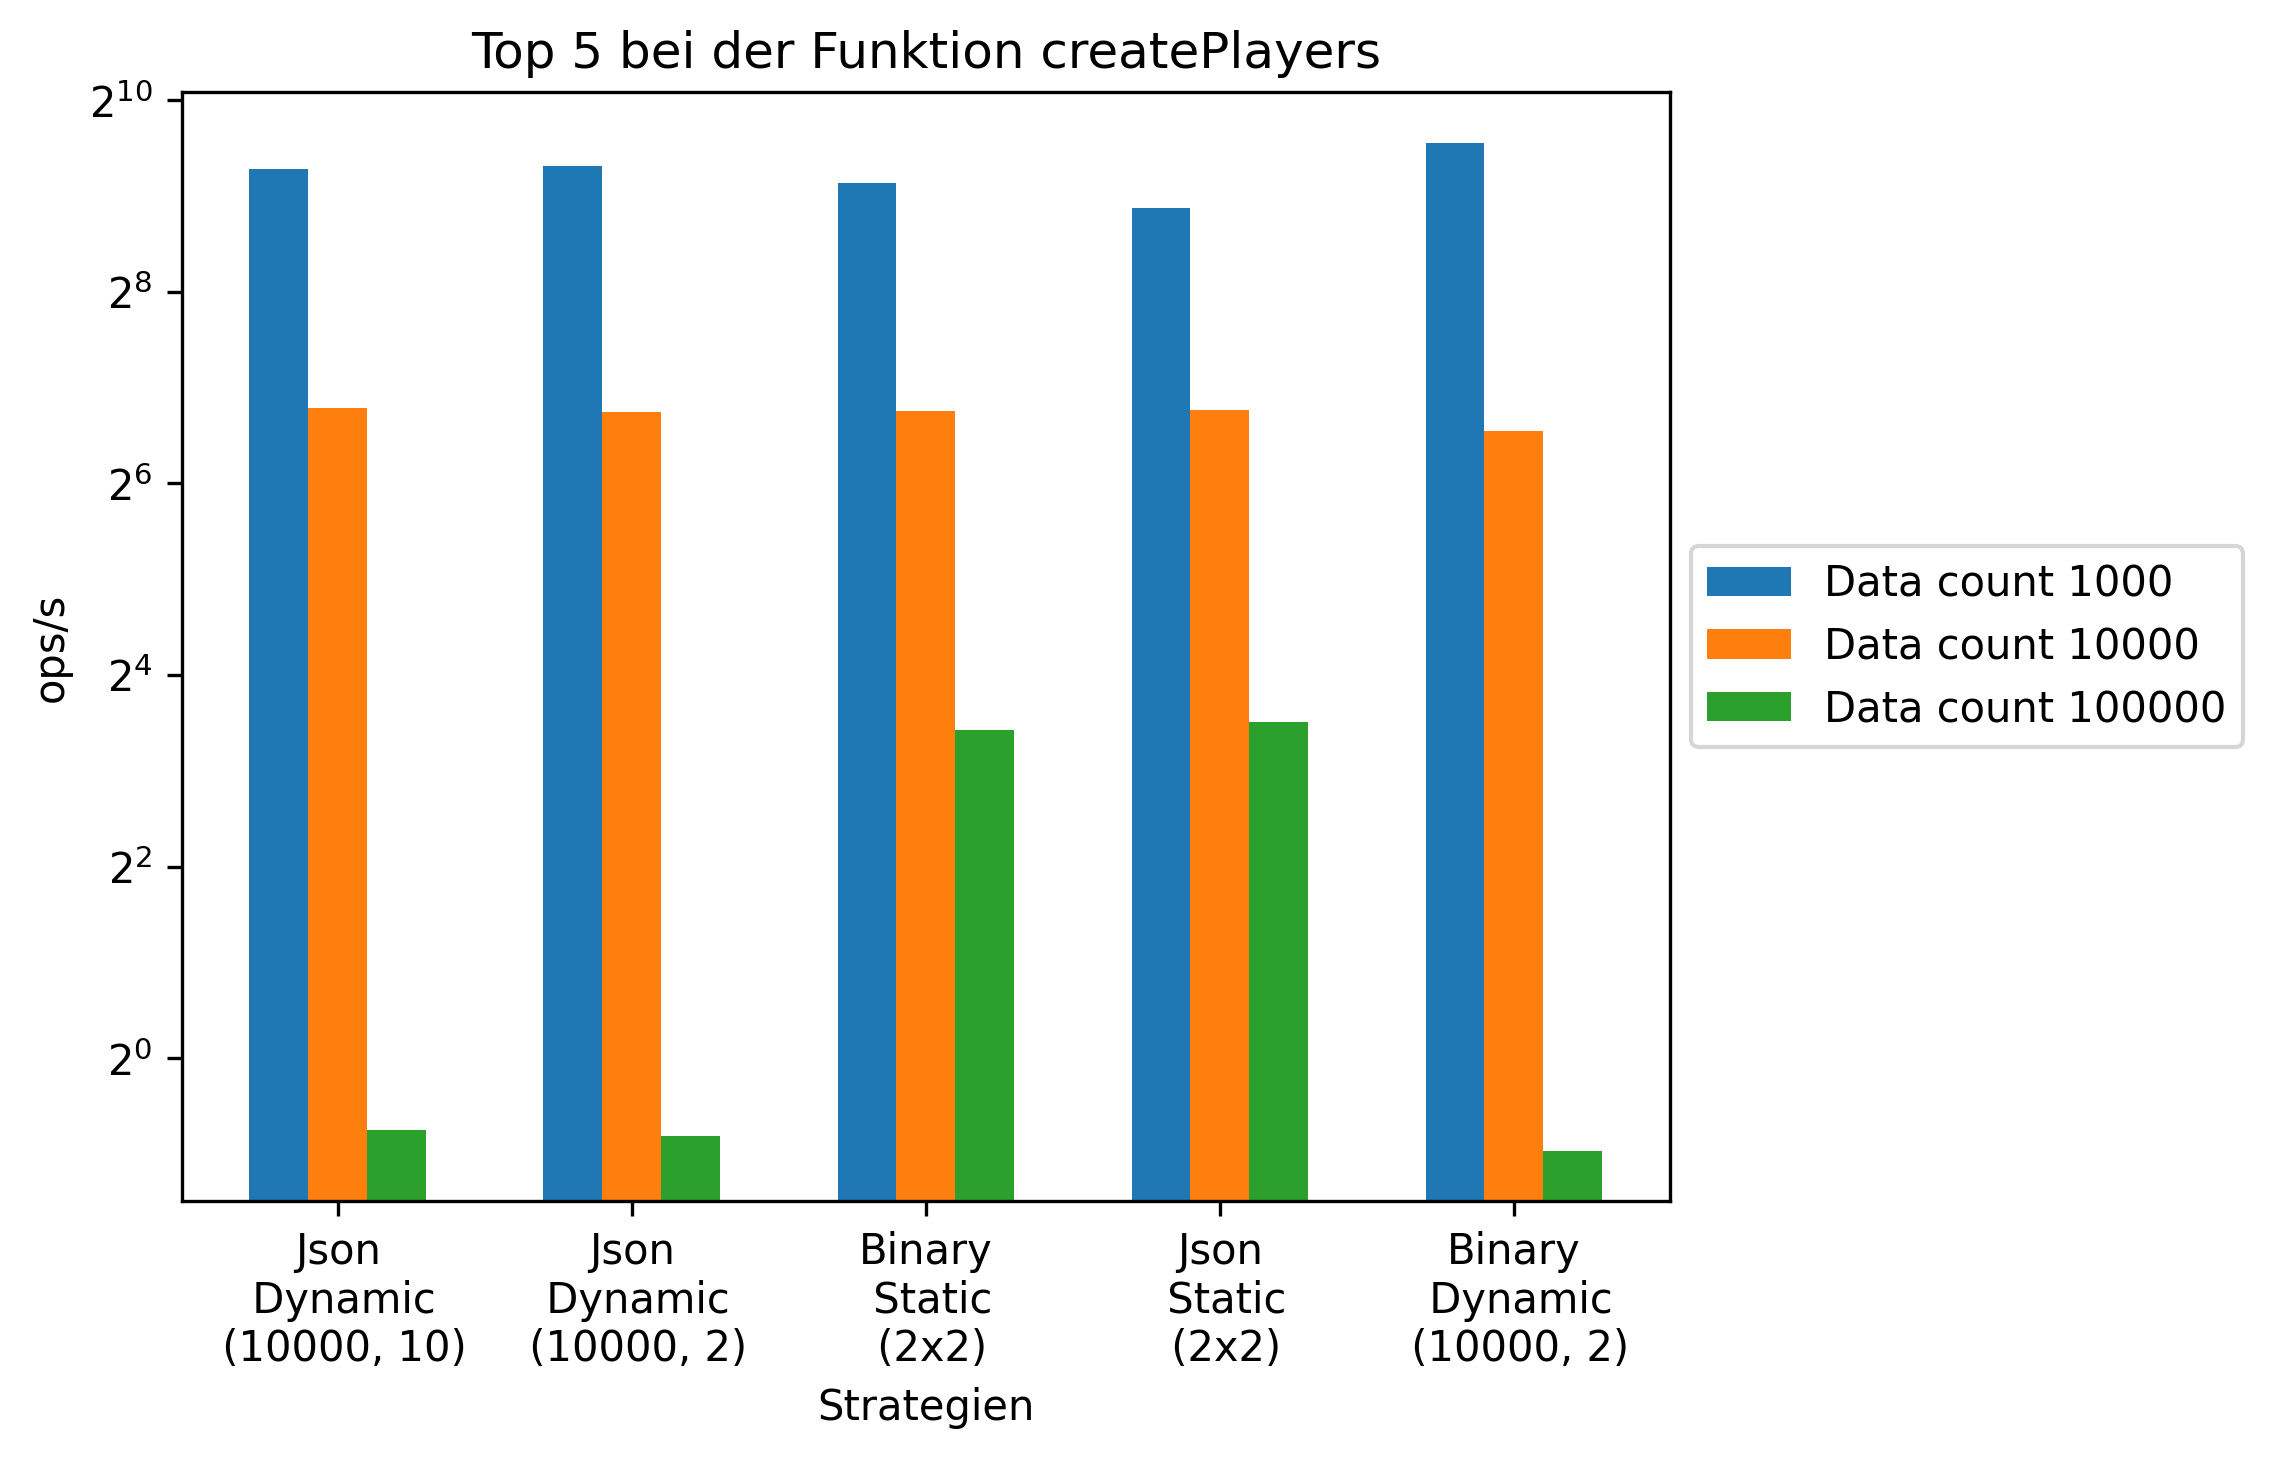
\includegraphics[width=0.7\textwidth]{images/plots/createPlayers.png}
    \caption{Beste Strategien für die Funktion createPlayers}
    \label{fig:createPlayers}
\end{figure}

\begin{figure}[htp]
    \centering
    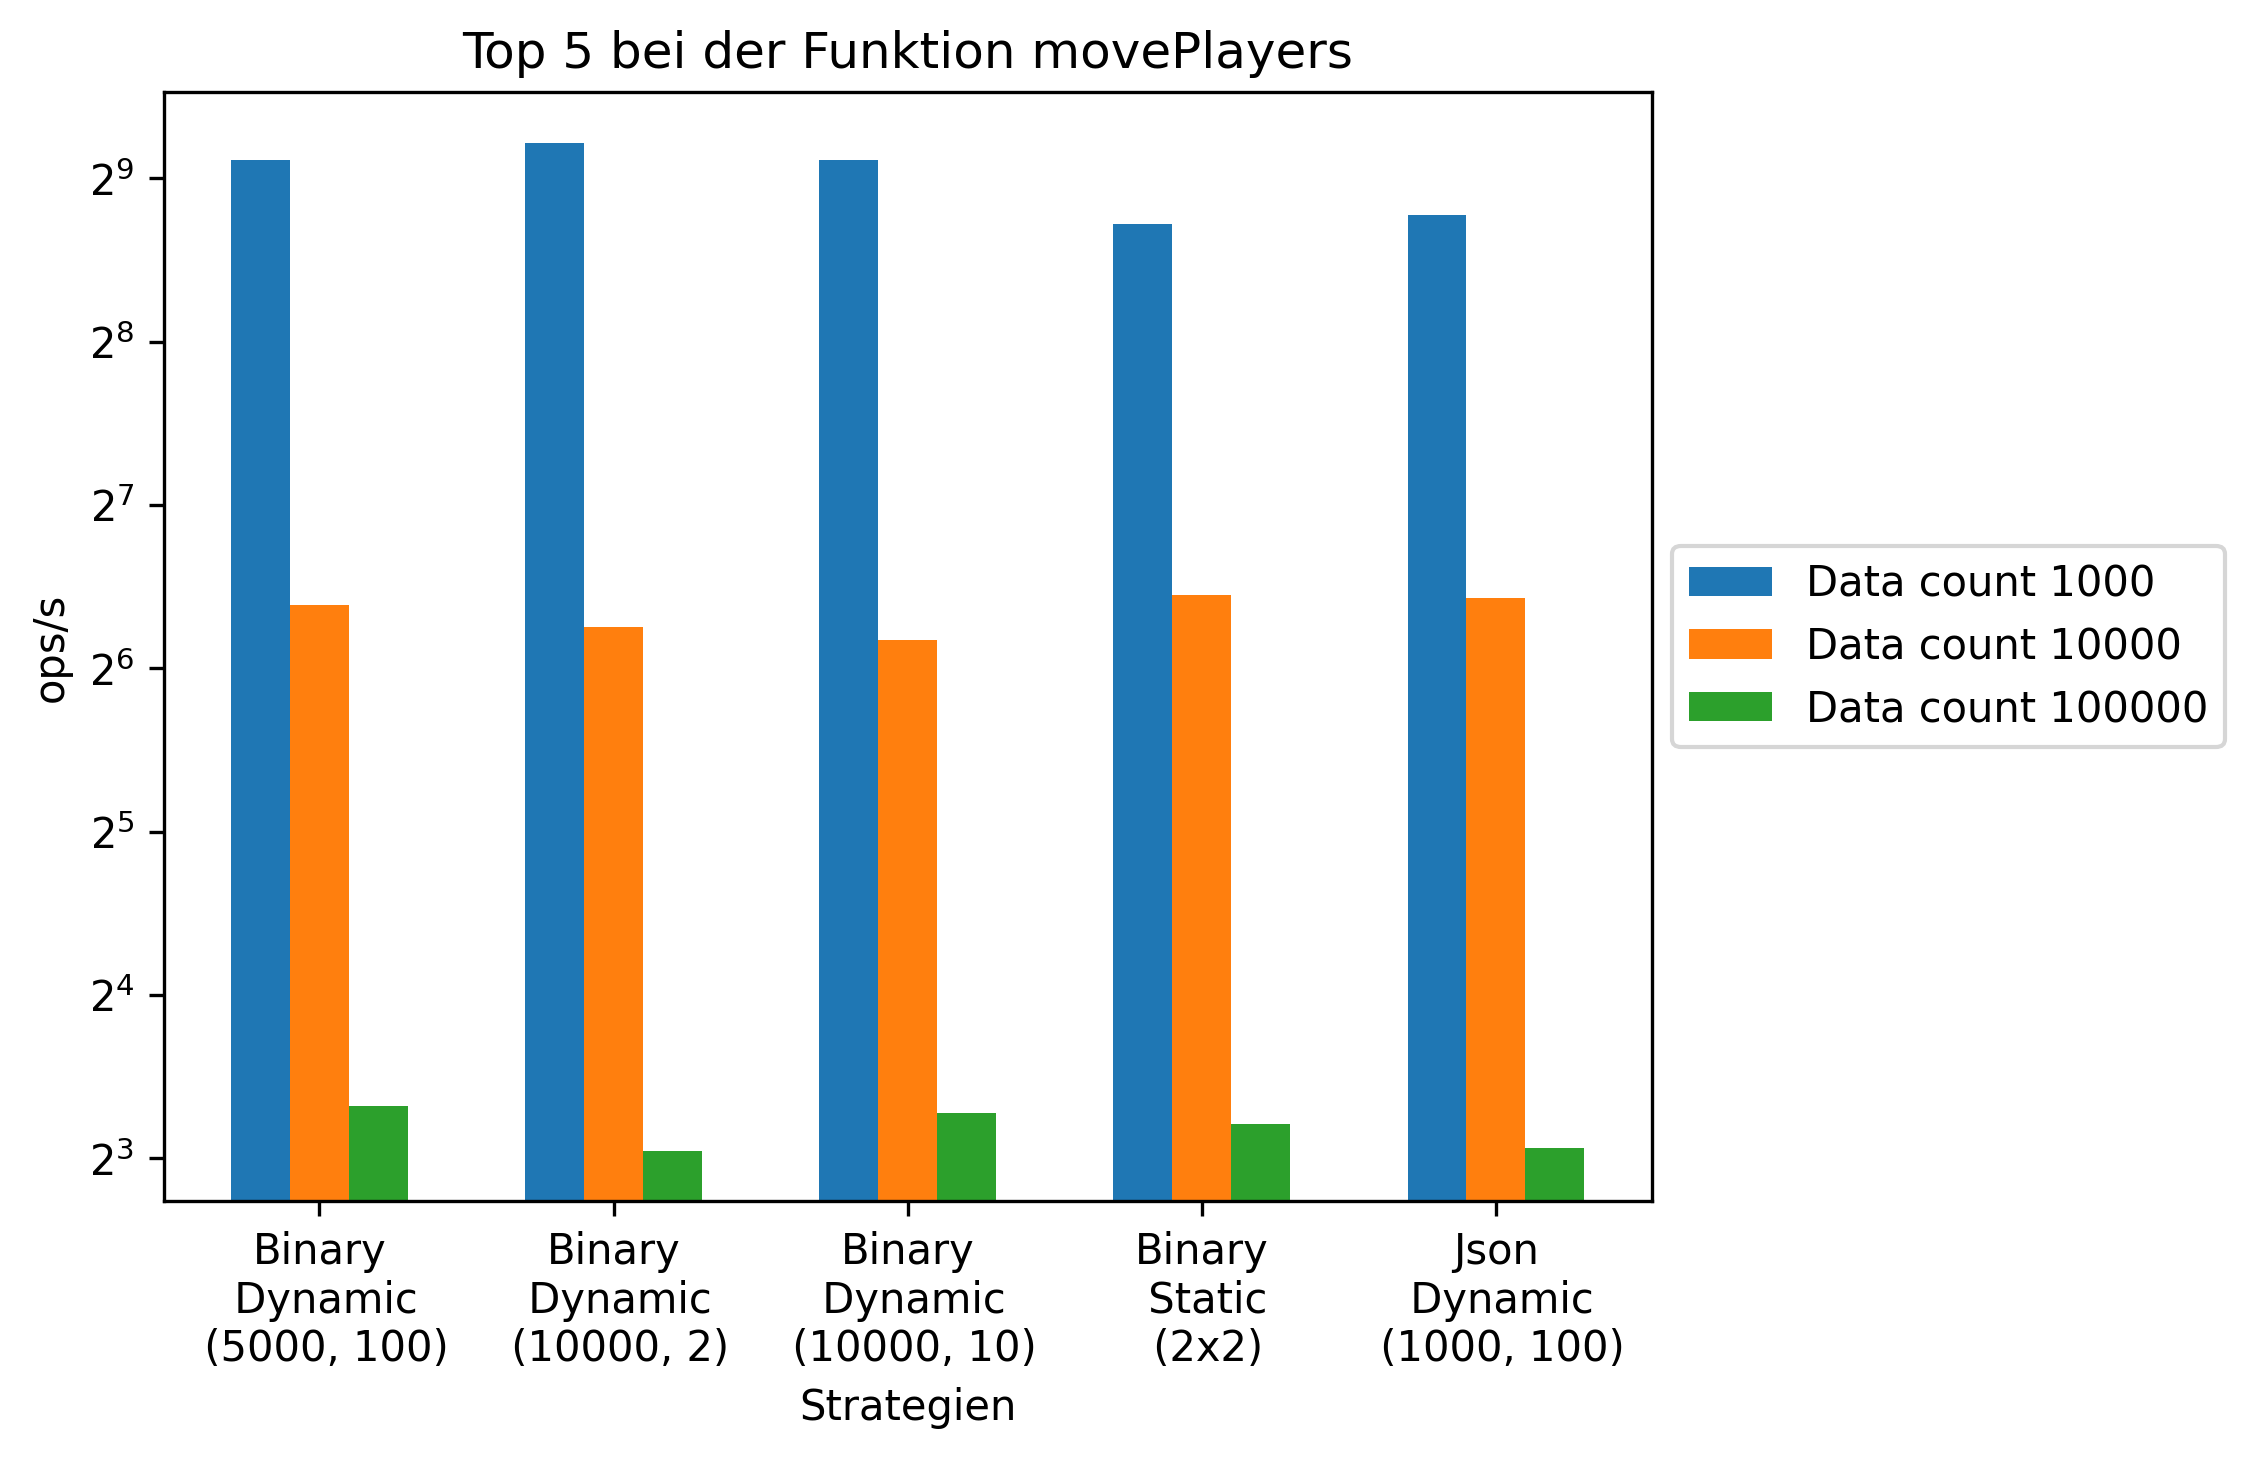
\includegraphics[width=0.7\textwidth]{images/plots/movePlayers.png}
    \caption{Beste Strategien für die Funktion movePlayers}
    \label{fig:movePlayers}
\end{figure}

\begin{figure}[htp]
    \centering
    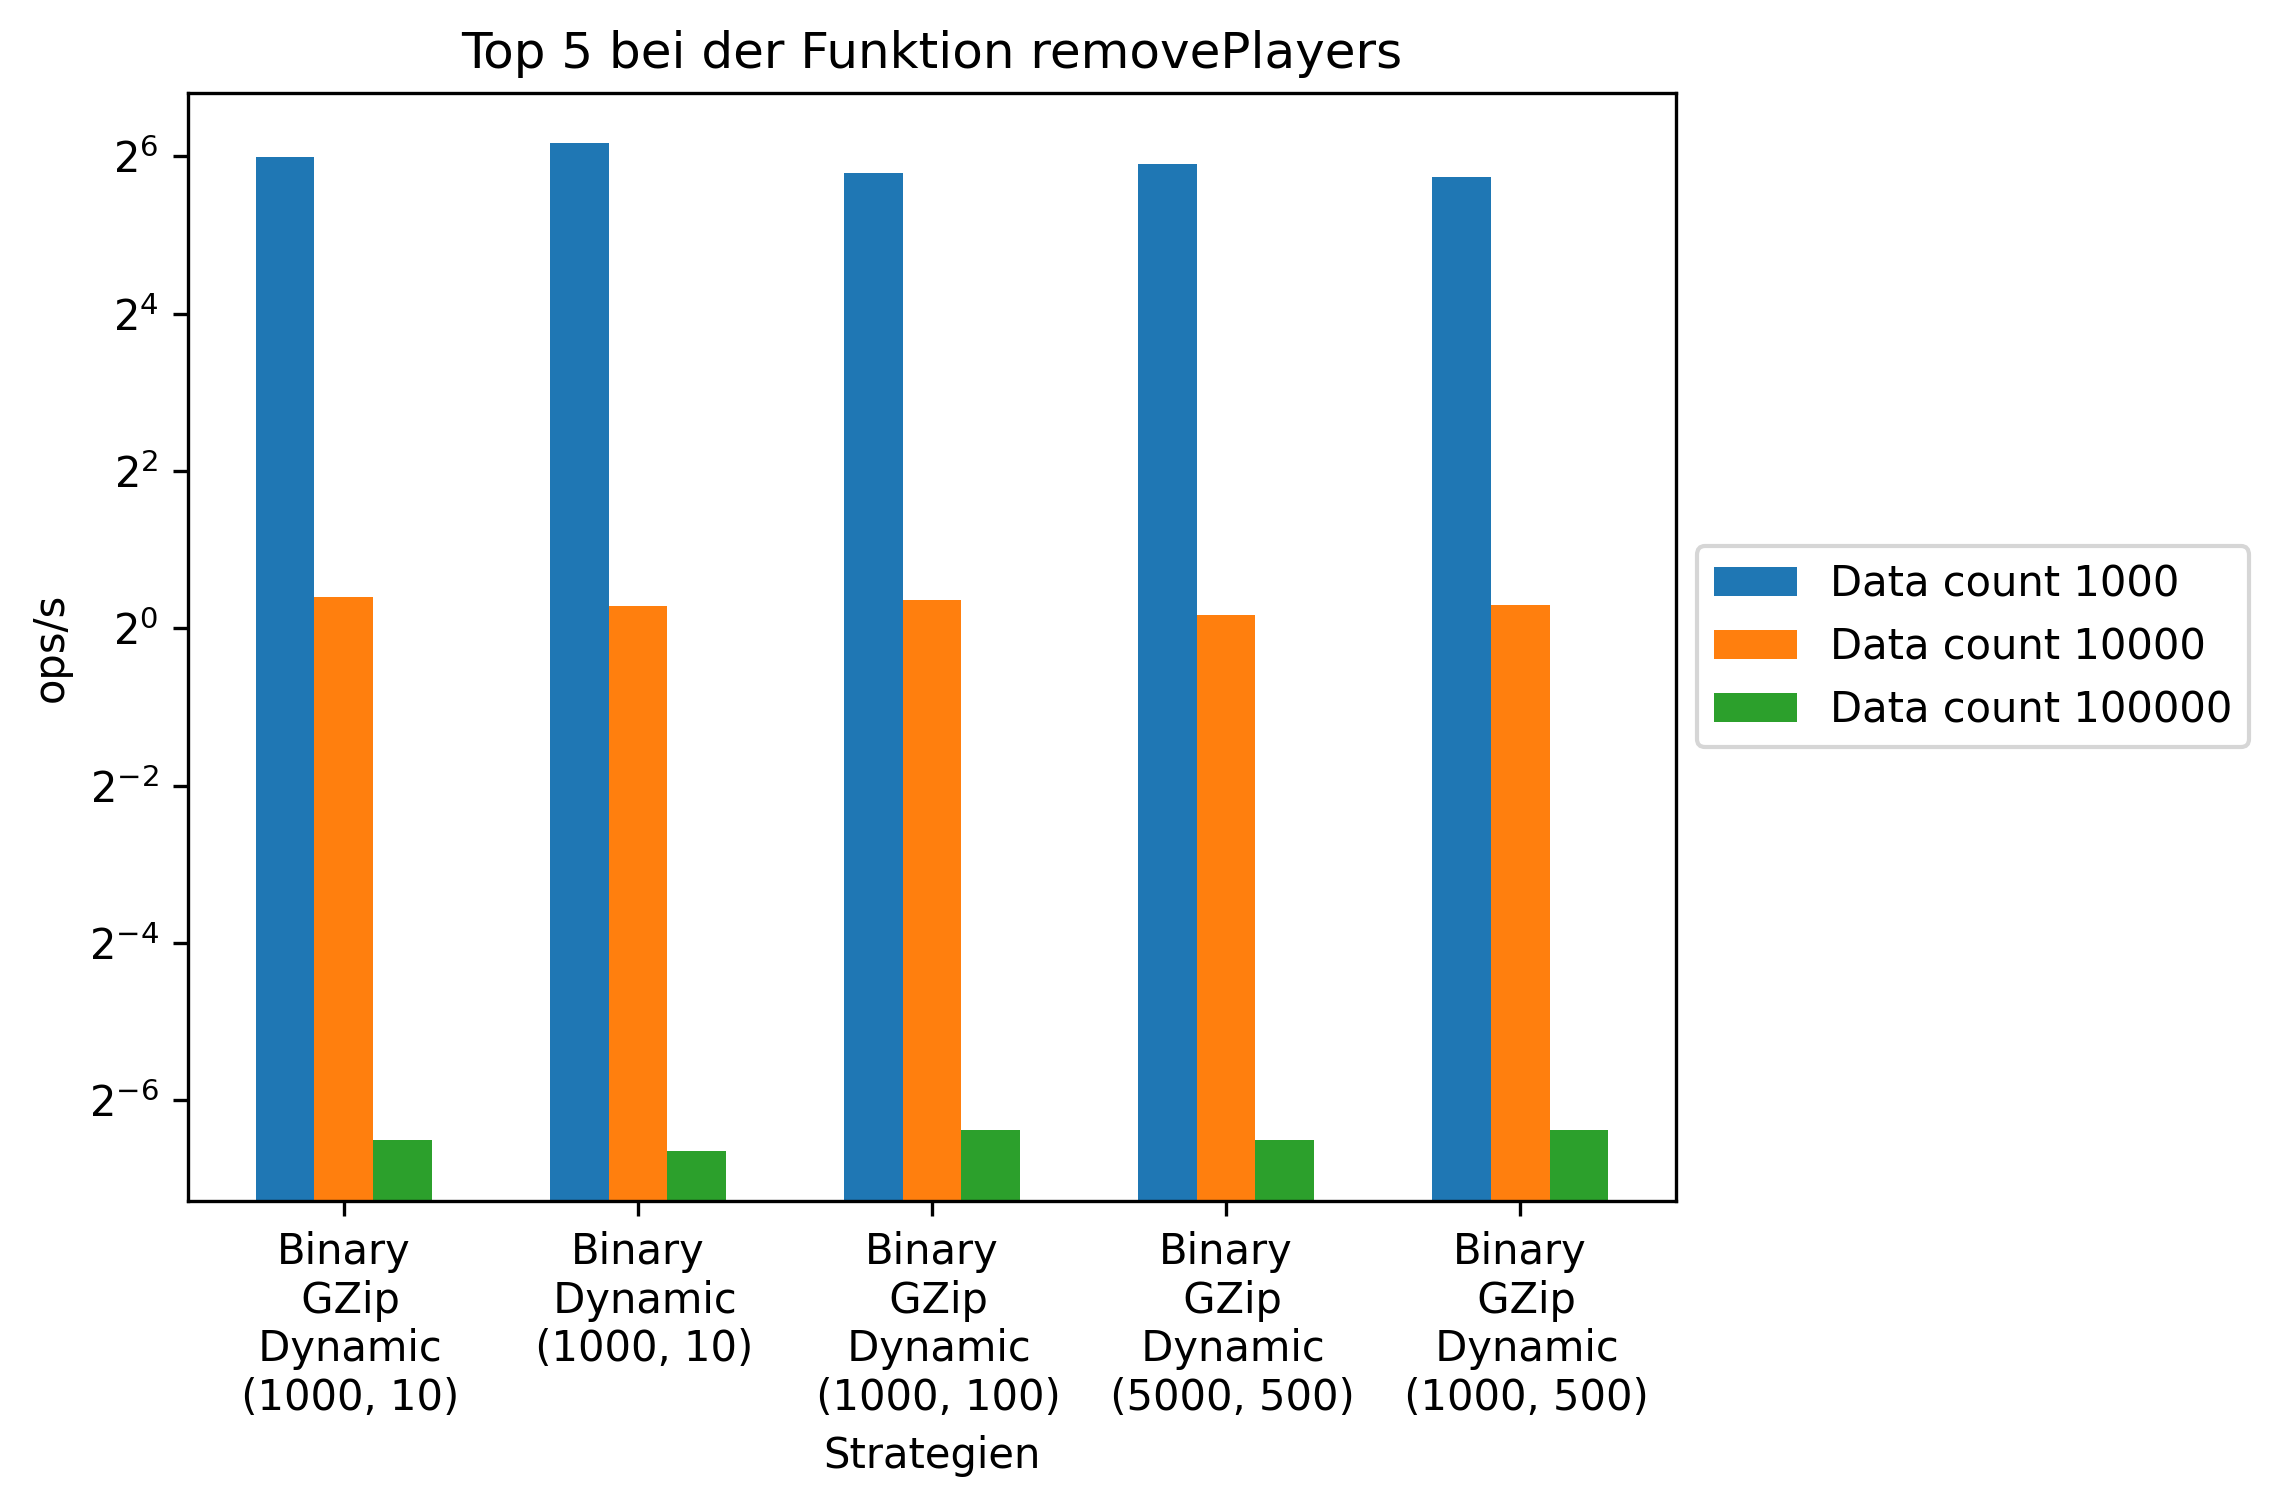
\includegraphics[width=0.7\textwidth]{images/plots/removePlayers.png}
    \caption{Beste Strategien für die Funktion removePlayers}
    \label{fig:removePlayers}
\end{figure}

\begin{figure}[htp]
    \centering
    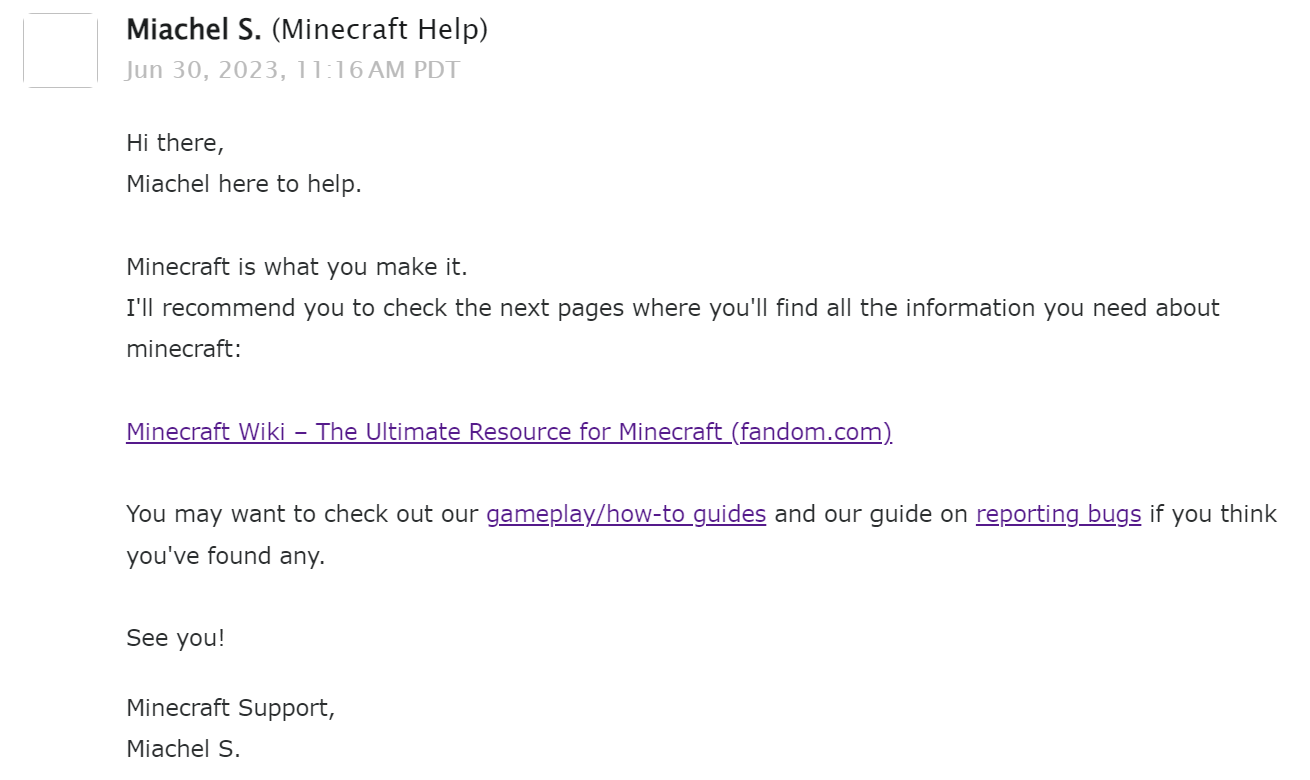
\includegraphics[width=1\textwidth]{images/Minecraft_Email.png}
    \caption{Email von Minecraft zu dem Speicher- und Ladesystem}
    \label{fig:minecraftMail}
\end{figure}

\begin{figure}[htp]
    \centering
    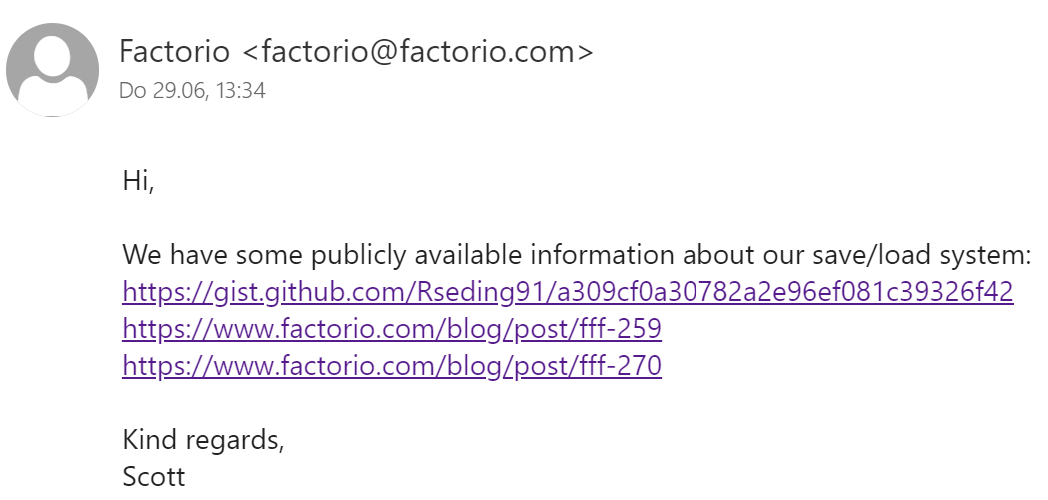
\includegraphics[width=1\textwidth]{images/Factorio_Email.png}
    \caption{Email von Factorio zu dem Speicher- und Ladesystem}
    \label{fig:factorioMail}
\end{figure}
